% Supplementary Appendix
% Cost-Effectiveness of Intismeran plus Pembrolizumab in Adjuvant Melanoma
% Yichao Jin, PhD
% PharmacoEconomics

\documentclass[11pt,a4paper]{article}
\usepackage[margin=1in]{geometry}
\usepackage{booktabs,graphicx,amsmath,hyperref,float,caption,tabularx,pdflscape,longtable}
\usepackage[numbers,sort&compress]{natbib}
\usepackage{tikz}
\usetikzlibrary{arrows.meta,positioning}
\bibliographystyle{unsrtnat}
\renewcommand{\thefigure}{S\arabic{figure}}
\renewcommand{\thetable}{S\arabic{table}}

\title{Supplementary Appendix\\
\large Cost-Effectiveness of Intismeran Autogene (mRNA-4157/V940) plus Pembrolizumab\\
versus Pembrolizumab Alone as Adjuvant Therapy for Resected Stage IIIB--IV Melanoma}
\author{Yichao Jin, PhD}
\date{}

\begin{document}
\maketitle
\tableofcontents
\newpage

% ═══════════════════════════════════════════════════
\section{Model Structure and Assumptions}
% ═══════════════════════════════════════════════════

\subsection{Health-State Definitions}
\label{sec:s1}
\begin{table}[H]
\centering
\caption{Health-State Definitions, Clinical Interpretation, and Model Inputs}
\label{tab:s1}
\begin{tabular}{lp{5cm}cc}
\toprule
\textbf{State} & \textbf{Clinical Definition} & \textbf{Utility} & \textbf{Monthly Cost} \\
\midrule
RF & Recurrence-free after complete resection; receiving adjuvant pembrolizumab (up to 18 cycles) with or without intismeran (up to 9 doses) & 0.83 & \$0 \\
LR & Confirmed locoregional recurrence without distant metastasis; includes salvage surgery, re-treatment, and surveillance & 0.64 & \$3,000 \\
DM & Confirmed stage IV melanoma with distant metastasis; includes systemic therapy, palliative care, and monitoring & 0.55 & \$12,000 \\
Death & All-cause mortality & 0 & \$0 \\
\bottomrule
\end{tabular}
\end{table}
\noindent\textit{Note:} Utilities and costs are drawn from published melanoma CEA literature \cite{bensimon2019, johnston2021, zhang2023}. Costs are in 2026 USD. See Supplementary Table~S9 for full PSA distribution parameters.

\subsection{State Occupancy Equations}
\label{sec:s2}
State occupancy at each monthly cycle is determined by the partitioned survival model (PSM) approach, using three parametric survival functions:

\begin{itemize}
    \item \textbf{RFS(t)} --- Recurrence-free survival: probability of remaining alive and free of any recurrence (locoregional or distant) at time $t$.
    \item \textbf{DMFS(t)} --- Distant metastasis-free survival: probability of remaining alive and free of distant metastasis at time $t$.
    \item \textbf{OS(t)} --- Overall survival: probability of being alive at time $t$.
\end{itemize}

The occupancy equations are derived from the ordering of these three events:
\begin{itemize}
    \item All patients who are recurrence-free are also distant metastasis-free and alive: $RF = RFS$.
    \item Patients who have had a locoregional recurrence but have not yet developed distant metastasis are those who are distant metastasis-free minus those who are recurrence-free: $LR = DMFS - RFS$.
    \item Patients who are alive with distant metastasis are those who are alive minus those who are distant metastasis-free: $DM = OS - DMFS$.
    \item The dead state is the complement of overall survival: $Dead = 1 - OS$.
\end{itemize}

The constraint $RFS \leq DMFS \leq OS$ is enforced at all time points to ensure non-negative state occupancy. This ordering is clinically meaningful: a patient cannot have distant metastasis without having had a recurrence event (RFS $\leq$ DMFS), and a patient cannot die without having both events (DMFS $\leq$ OS). The ratio-constrained structure $r_{\text{LR}} = RFS/DMFS$ and $r_{\text{DM}} = DMFS/OS$ guarantees this ordering by construction.

\subsection{Model Schematic}
\label{sec:s1diagram}
\begin{figure}[H]
\centering
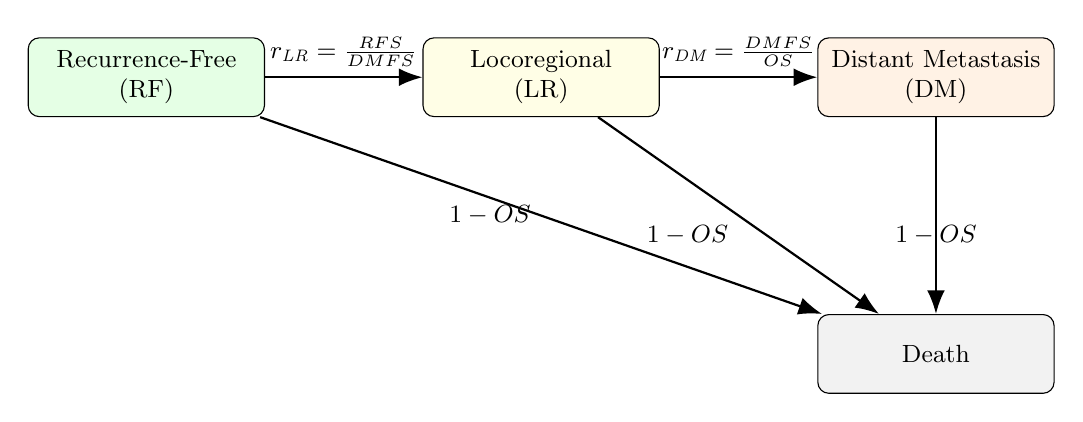
\begin{tikzpicture}[
  node distance=1.5cm and 2cm,
  box/.style={draw, rectangle, rounded corners, minimum width=3cm, minimum height=1cm, align=center, font=\small},
  arrow/.style={-{Latex[length=3mm]}, thick},
  label/.style={font=\small\itshape}
]
  \node[box,fill=green!10] (rf) {Recurrence-Free\\(RF)};
  \node[box,fill=yellow!10,right=of rf] (lr) {Locoregional\\(LR)};
  \node[box,fill=orange!10,right=of lr] (dm) {Distant Metastasis\\(DM)};
  \node[box,fill=gray!10,below=2.5cm of dm] (dead) {Death};

  \draw[arrow] (rf) -- node[above,label]{$r_{\text{LR}} = \frac{RFS}{DMFS}$} (lr);
  \draw[arrow] (lr) -- node[above,label]{$r_{\text{DM}} = \frac{DMFS}{OS}$} (dm);
  \draw[arrow] (rf) -- node[left,label]{$1 - OS$} (dead);
  \draw[arrow] (lr) -- node[below left,label]{$1 - OS$} (dead);
  \draw[arrow] (dm) -- node[below,label]{$1 - OS$} (dead);
\end{tikzpicture}
\caption{Partitioned survival model structure. The model uses four mutually exclusive health states. State occupancy is derived from three parametric survival functions (RFS, DMFS, OS) rather than from transition probabilities. Arrows denote the ratio-constrained relationship $RFS \leq DMFS \leq OS$.}
\label{fig:s1}
\end{figure}

% ═══════════════════════════════════════════════════
\section{Survival Data and Parametric Extrapolation}
% ═══════════════════════════════════════════════════

\subsection{Extracted Survival Probabilities}
\label{sec:survival_data}

Survival probabilities were extracted from the published Kaplan--Meier curves (Figure~1) of Khattak et al.\ (2026) \cite{khattak2026} using WebPlotDigitizer v4.7. Data were extracted at 18, 24, 36, 48, and 60 months for OS and RFS, and at 18, 24, 36, and 48 months for DMFS. The extracted values are reported in Table~\ref{tab:s2}.

\begin{table}[H]
\centering
\caption{Extracted KEYNOTE-942 Survival Probabilities (\%)}
\label{tab:s2}
\begin{tabular}{lcccccc}
\toprule
\textbf{Month} & \multicolumn{2}{c}{\textbf{RFS (\%)}} & \multicolumn{2}{c}{\textbf{DMFS (\%)}} & \multicolumn{2}{c}{\textbf{OS (\%)}} \\
\cmidrule(lr){2-3} \cmidrule(lr){4-5} \cmidrule(lr){6-7}
 & Combo & Pembro & Combo & Pembro & Combo & Pembro \\
\midrule
18 & 80.4 & 62.2 & 92.0 & 73.0 & 96.0 & 93.4 \\
24 & 78.3 & 60.0 & 90.8 & 70.6 & 96.0 & 93.4 \\
36 & 73.8 & 55.6 & 85.6 & 65.4 & 93.8 & 85.6 \\
48 & 72.4 & 49.1 & 83.9 & 65.4 & 92.2 & 85.6 \\
60 & 68.8 & 49.1 & --- & --- & 92.2 & 71.3 \\
\bottomrule
\end{tabular}
\end{table}

\noindent\textbf{Digitization method:} WebPlotDigitizer v4.7, manual extraction. The 60-month landmark values match the published 5-year ASCO 2026 update \cite{khattak2026}. At earlier time points, the 18-month RFS rates from the primary analysis \cite{weber2024} differ from digitized values by 1.4 pp (combo) and 0.2 pp (pembro), consistent with typical digitization error. The 5-year RFS 95\% CIs: combo 56.3--78.3\%, pembro 33.3--63.0\%.

% ═══════════════════════════════════════════════════
\section{Clinical Input Provenance}
% ═══════════════════════════════════════════════════
\label{sec:provenance}

Table~\ref{tab:provenance} summarizes the provenance of all clinical inputs used in the model. The evidence status column classifies each input into one of five categories:

\begin{itemize}
    \item \textbf{Published:} The value is directly reported in the cited source.
    \item \textbf{Digitized:} The value was extracted from a published Kaplan--Meier curve using WebPlotDigitizer v4.7.
    \item \textbf{Derived:} The value is mathematically derived from other inputs (e.g., ratio of survival functions).
    \item \textbf{Modeled:} The value is produced by the model's parametric extrapolation (e.g., long-term survival beyond observed data).
    \item \textbf{Topline only:} The source reports a statistically significant result but the numerical hazard ratio or landmark survival probabilities have not yet been disclosed.
\end{itemize}

\small
\begin{longtable}{>{\raggedright\arraybackslash}p{5cm}p{2.2cm}p{2.4cm}p{4cm}}
\caption{Clinical Input Provenance}\\
\label{tab:provenance}\\
\toprule
\textbf{Input} & \textbf{Value} & \textbf{Evidence} & \textbf{Source} \\
& & \textbf{Status} & \\
\midrule
\endfirsthead
\toprule
\textbf{Input} & \textbf{Value} & \textbf{Evidence} & \textbf{Source} \\
& & \textbf{Status} & \\
\midrule
\endhead
\bottomrule
\endlastfoot
\toprule
\textbf{Input} & \textbf{Value} & \textbf{Evidence} & \textbf{Source} \\
& & \textbf{Status} & \\
\midrule
\multicolumn{4}{c}{\textit{KEYNOTE-942 (Phase 2b, 5-year follow-up)}} \\
\midrule
\multicolumn{4}{l}{\textbf{Recurrence-Free Survival (RFS)}} \\
\quad 18-month RFS, combo & 80.4\% & Digitized & Fig.~1, Khattak 2026 \\
\quad 24-month RFS, combo & 78.3\% & Digitized & Fig.~1, Khattak 2026 \\
\quad 36-month RFS, combo & 73.8\% & Digitized & Fig.~1, Khattak 2026 \\
\quad 48-month RFS, combo & 72.4\% & Digitized & Fig.~1, Khattak 2026 \\
\quad 60-month RFS, combo & 68.8\% & Published & Khattak 2026 \\
\quad 60-month RFS, combo 95\% CI & 56.3--78.3\% & Published & Khattak 2026 \\
\quad 18-month RFS, pembro & 62.2\% & Digitized & Fig.~1, Khattak 2026 \\
\quad 24-month RFS, pembro & 60.0\% & Digitized & Fig.~1, Khattak 2026 \\
\quad 36-month RFS, pembro & 55.6\% & Digitized & Fig.~1, Khattak 2026 \\
\quad 48-month RFS, pembro & 49.1\% & Digitized & Fig.~1, Khattak 2026 \\
\quad 60-month RFS, pembro & 49.1\% & Published & Khattak 2026 \\
\quad 60-month RFS, pembro 95\% CI & 33.3--63.0\% & Published & Khattak 2026 \\
\midrule
\multicolumn{4}{l}{\textbf{Distant Metastasis-Free Survival (DMFS)}} \\
\quad 18-month DMFS, combo & 92.0\% & Digitized & Fig.~1, Khattak 2026 \\
\quad 24-month DMFS, combo & 90.8\% & Digitized & Fig.~1, Khattak 2026 \\
\quad 36-month DMFS, combo & 85.6\% & Digitized & Fig.~1, Khattak 2026 \\
\quad 48-month DMFS, combo & 83.9\% & Digitized & Fig.~1, Khattak 2026 \\
\quad 60-month DMFS, combo & -- & Not reported & N/A \\
\quad 18-month DMFS, pembro & 73.0\% & Digitized & Fig.~1, Khattak 2026 \\
\quad 24-month DMFS, pembro & 70.6\% & Digitized & Fig.~1, Khattak 2026 \\
\quad 36-month DMFS, pembro & 65.4\% & Digitized & Fig.~1, Khattak 2026 \\
\quad 48-month DMFS, pembro & 65.4\% & Digitized & Fig.~1, Khattak 2026 \\
\quad 60-month DMFS, pembro & -- & Not reported & N/A \\
\midrule
\multicolumn{4}{l}{\textbf{Overall Survival (OS)}} \\
\quad 18-month OS, combo & 96.0\% & Digitized & Fig.~1, Khattak 2026 \\
\quad 24-month OS, combo & 96.0\% & Digitized & Fig.~1, Khattak 2026 \\
\quad 36-month OS, combo & 93.8\% & Digitized & Fig.~1, Khattak 2026 \\
\quad 48-month OS, combo & 92.2\% & Published & Khattak 2026 \\
\quad 60-month OS, combo & 92.2\% & Published & Khattak 2026 \\
\quad 18-month OS, pembro & 93.4\% & Digitized & Fig.~1, Khattak 2026 \\
\quad 24-month OS, pembro & 93.4\% & Digitized & Fig.~1, Khattak 2026 \\
\quad 36-month OS, pembro & 85.6\% & Digitized & Fig.~1, Khattak 2026 \\
\quad 48-month OS, pembro & 85.6\% & Published & Khattak 2026 \\
\quad 60-month OS, pembro & 71.3\% & Published & Khattak 2026 \\
\midrule
\multicolumn{4}{l}{\textbf{Hazard Ratios}} \\
\quad RFS HR (combo vs. pembro) & 0.510 & Published & Khattak 2026 \\
\quad RFS HR 95\% CI & 0.294--0.887 & Published & Khattak 2026 \\
\quad DMFS HR (combo vs. pembro) & 0.411 & Published & Khattak 2026 \\
\quad DMFS HR 95\% CI & 0.200--0.843 & Published & Khattak 2026 \\
\quad OS HR (combo vs. pembro) & 0.471 & Published & Khattak 2026 \\
\quad OS HR 95\% CI & 0.165--1.345 & Published & Khattak 2026 \\
\quad OS events & 14 (7 per arm) & Published & Khattak 2026 \\
\midrule
\multicolumn{4}{c}{\textit{INTerpath-001 (Phase 3, topline announcement)}} \\
\midrule
\quad RFS & Statistically significant & Topline only & Merck/Moderna 2026 \\
\quad DMFS & Statistically significant & Topline only & Merck/Moderna 2026 \\
\quad Numerical HR / KM curves & Not yet disclosed & Topline only & N/A \\
\midrule
\multicolumn{4}{c}{\textit{Modeled / Derived Values}} \\
\midrule
\multicolumn{4}{l}{\textbf{Fitted log-normal parameters}} \\
\quad OS $\mu$ (combo), $\sigma$ (combo) & 4.825, 0.879 & Derived & Least-squares fit \\
\quad OS $\mu$ (pembro), $\sigma$ (pembro) & 4.214, 1.332 & Derived & Least-squares fit \\
\quad r\_DM $\mu$ (combo), $\sigma$ (combo) & 4.285, 0.851 & Derived & Ratio fit \\
\quad r\_DM $\mu$ (pembro), $\sigma$ (pembro) & 3.475, 1.390 & Derived & Ratio fit \\
\quad r\_LR $\mu$ (combo), $\sigma$ (combo) & 3.420, 1.250 & Derived & Ratio fit \\
\quad r\_LR $\mu$ (pembro), $\sigma$ (pembro) & 2.268, 1.749 & Derived & Ratio fit \\
\midrule
\multicolumn{4}{l}{\textbf{Long-term extrapolation}} \\
\quad 10-year OS, combo & 74.4\% & Modeled & Log-normal extrapolation \\
\quad 10-year OS, pembro & 46.3\% & Modeled & Log-normal extrapolation \\
\quad 20-year OS, combo (GP-constrained) & 18.3\% & Modeled & GP hazard floor \\
\quad 20-year OS, pembro (GP-constrained) & 7.8\% & Modeled & GP hazard floor \\
\quad 40-year OS, combo (GP-constrained) & 0.0\% & Modeled & GP hazard floor \\
\bottomrule
\bottomrule
\end{longtable}

\subsection{Observed vs.\ Fitted Survival Curves}
\label{sec:obs_vs_fitted}
\begin{figure}[H]
\centering
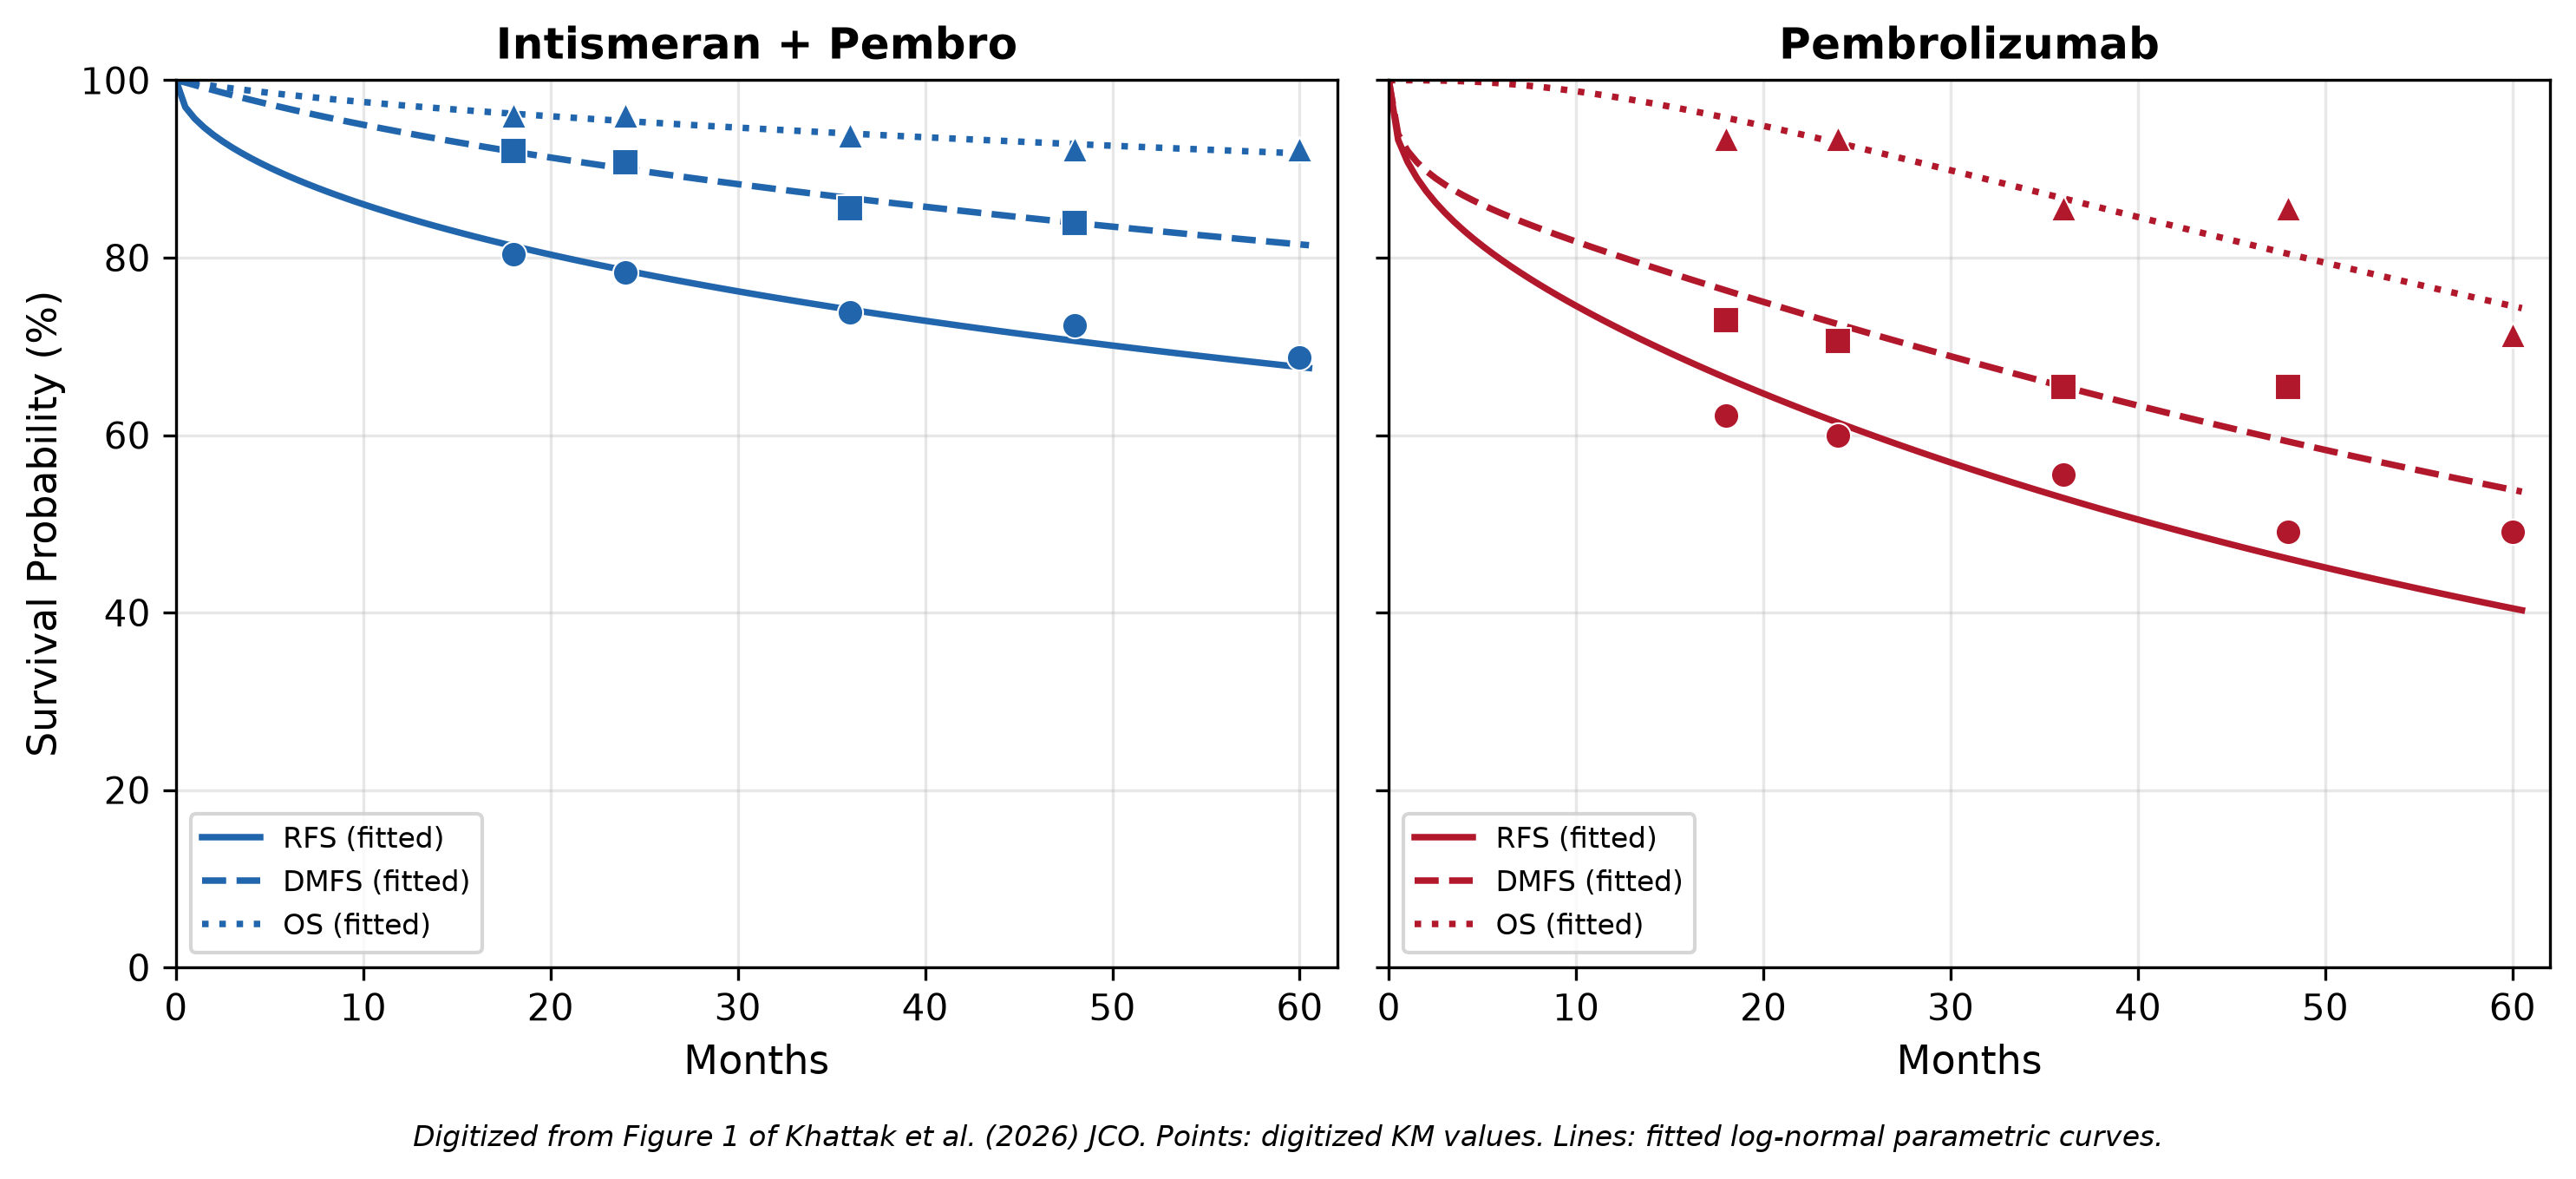
\includegraphics[width=\textwidth]{fig_s2_survival_data.png}
\caption{Digitized KEYNOTE-942 survival data (points) and fitted log-normal parametric curves (lines). Left panel: intismeran plus pembrolizumab arm. Right panel: pembrolizumab alone arm.}
\label{fig:s2}
\end{figure}

% ═══════════════════════════════════════════════════
\section{Survival Model Selection}
% ═══════════════════════════════════════════════════

\subsection{Component-Level Parametric Fit}
\label{sec:s3}
\begin{table}[H]
\centering
\caption{Component-Level Parametric Fit Across Five Distributions}
\label{tab:s3}
\begin{tabular}{lcccc}
\toprule
\textbf{Component} & \textbf{Distribution} & \textbf{AIC} & \textbf{RMSE} & \textbf{Rank} \\
\midrule
\multicolumn{5}{c}{\textit{OS -- Combo arm}} \\
Exponential & 1 param & -45.49 & 0.0087 & 4 \\
Weibull & 2 param & -49.84 & 0.0046 & 2 \\
Log-normal & 2 param & -50.08 & 0.0045 & 1 \\
Log-logistic & 2 param & -49.89 & 0.0046 & 3 \\
Generalized gamma & 3 param & -47.97 & 0.0045 & 5 \\
\midrule
\multicolumn{5}{c}{\textit{OS -- Pembro arm}} \\
Exponential & 1 param & -31.27 & 0.0359 & 4 \\
Weibull & 2 param & -32.00 & 0.0273 & 1 \\
Log-normal & 2 param & -31.16 & 0.0297 & 3 \\
Log-logistic & 2 param & -31.69 & 0.0282 & 2 \\
Generalized gamma & 3 param & -30.33 & 0.0264 & 5 \\
\midrule
\multicolumn{5}{c}{\textit{r$_{\text{DM}}$ -- Combo arm}} \\
Exponential & 1 param & -36.79 & 0.0078 & 3 \\
Weibull & 2 param & -36.53 & 0.0063 & 4 \\
Log-normal & 2 param & -36.93 & 0.0060 & 1 \\
Log-logistic & 2 param & -36.61 & 0.0062 & 2 \\
Generalized gamma & 3 param & -34.74 & 0.0061 & 5 \\
\midrule
\multicolumn{5}{c}{\textit{r$_{\text{DM}}$ -- Pembro arm}} \\
Exponential & 1 param & -19.41 & 0.0688 & 5 \\
Weibull & 2 param & -28.43 & 0.0174 & 3 \\
Log-normal & 2 param & -27.23 & 0.0202 & 4 \\
Log-logistic & 2 param & -30.30 & 0.0137 & 2 \\
Generalized gamma & 3 param & -32.45 & 0.0082 & 1 \\
\midrule
\multicolumn{5}{c}{\textit{r$_{\text{LR}}$ -- Combo arm}} \\
Exponential & 1 param & -30.38 & 0.0392 & 5 \\
Weibull & 2 param & -38.97 & 0.0136 & 3 \\
Log-normal & 2 param & -39.49 & 0.0129 & 2 \\
Log-logistic & 2 param & -39.70 & 0.0126 & 1 \\
Generalized gamma & 3 param & -38.43 & 0.0118 & 4 \\
\midrule
\multicolumn{5}{c}{\textit{r$_{\text{LR}}$ -- Pembro arm}} \\
Exponential & 1 param & -31.82 & 0.0340 & 5 \\
Weibull & 2 param & -33.60 & 0.0233 & 1 \\
Log-normal & 2 param & -33.37 & 0.0238 & 2 \\
Log-logistic & 2 param & -33.51 & 0.0235 & 3 \\
Generalized gamma & 3 param & -31.69 & 0.0231 & 4 \\
\bottomrule
\end{tabular}
\end{table}

\subsection{Joint Model Selection}
\label{sec:joint}
A total of 4,096 distribution combinations were evaluated for structural validity at 40 years. All 4,096 satisfied the RFS $\leq$ DMFS $\leq$ OS ordering constraint (0 crossing violations). The full results are available online (\texttt{output/survival\_combos\_4096.csv}).

\begin{table}[H]
\centering
\caption{Top 10 Joint Model Combinations by Total AIC}
\label{tab:s4}
\begin{tabular}{lccccccc}
\toprule
\textbf{Rank} & \textbf{OS} & \textbf{r$_{\text{DM}}$} & \textbf{r$_{\text{LR}}$} & \textbf{Total AIC} & \textbf{OS40c} & \textbf{OS40p} \\
\cmidrule(lr){2-3} \cmidrule(lr){4-4} \cmidrule(lr){5-5} \cmidrule(lr){6-7}
 & C/P & C/P & C/P & & & \\
\midrule
1 & LN / W & LN / LL & LL / W & -222.61 & 76.3\% & 0.0\% \\
2 & LN / W & LN / LL & LL / LL & -222.52 & 76.3\% & 0.0\% \\
3 & LN / W & Exp / LL & LL / W & -222.47 & 76.3\% & 0.0\% \\
4 & LLog / W & LN / LL & LL / W & -222.42 & 72.9\% & 0.0\% \\
5 & LN / W & LN / LL & LN / W & -222.40 & 76.3\% & 0.0\% \\
6 & LN / W & LN / LL & LL / LN & -222.39 & 76.3\% & 0.0\% \\
7 & LN / W & Exp / LL & LL / LL & -222.38 & 76.3\% & 0.0\% \\
8 & W / W & LN / LL & LL / W & -222.37 & 71.1\% & 0.0\% \\
9 & LLog / W & LN / LL & LL / LL & -222.33 & 72.9\% & 0.0\% \\
10 & LN / W & LN / LL & LN / LL & -222.31 & 76.3\% & 0.0\% \\
\bottomrule
\end{tabular}
\end{table}
\noindent\textit{Distributions:} LN = log-normal, W = weibull, LLog = log-logistic, Exp = exponential. C/P = Combo/Pembro. All top-ranked combinations use log-normal OS for the combo arm, yielding OS40c = 71.1--76.3\% under unconstrained extrapolation, substantially higher than GP survival at age 101 ($\approx$0\%). This motivated the GP mortality hazard floor (Section~\ref{sec:gp_impl}), under which the constrained OS40c falls to 0.0\% for both arms.

\subsection{Lifetime OS Extrapolation by Distribution}
\label{sec:os_extrap}
\begin{figure}[H]
\centering
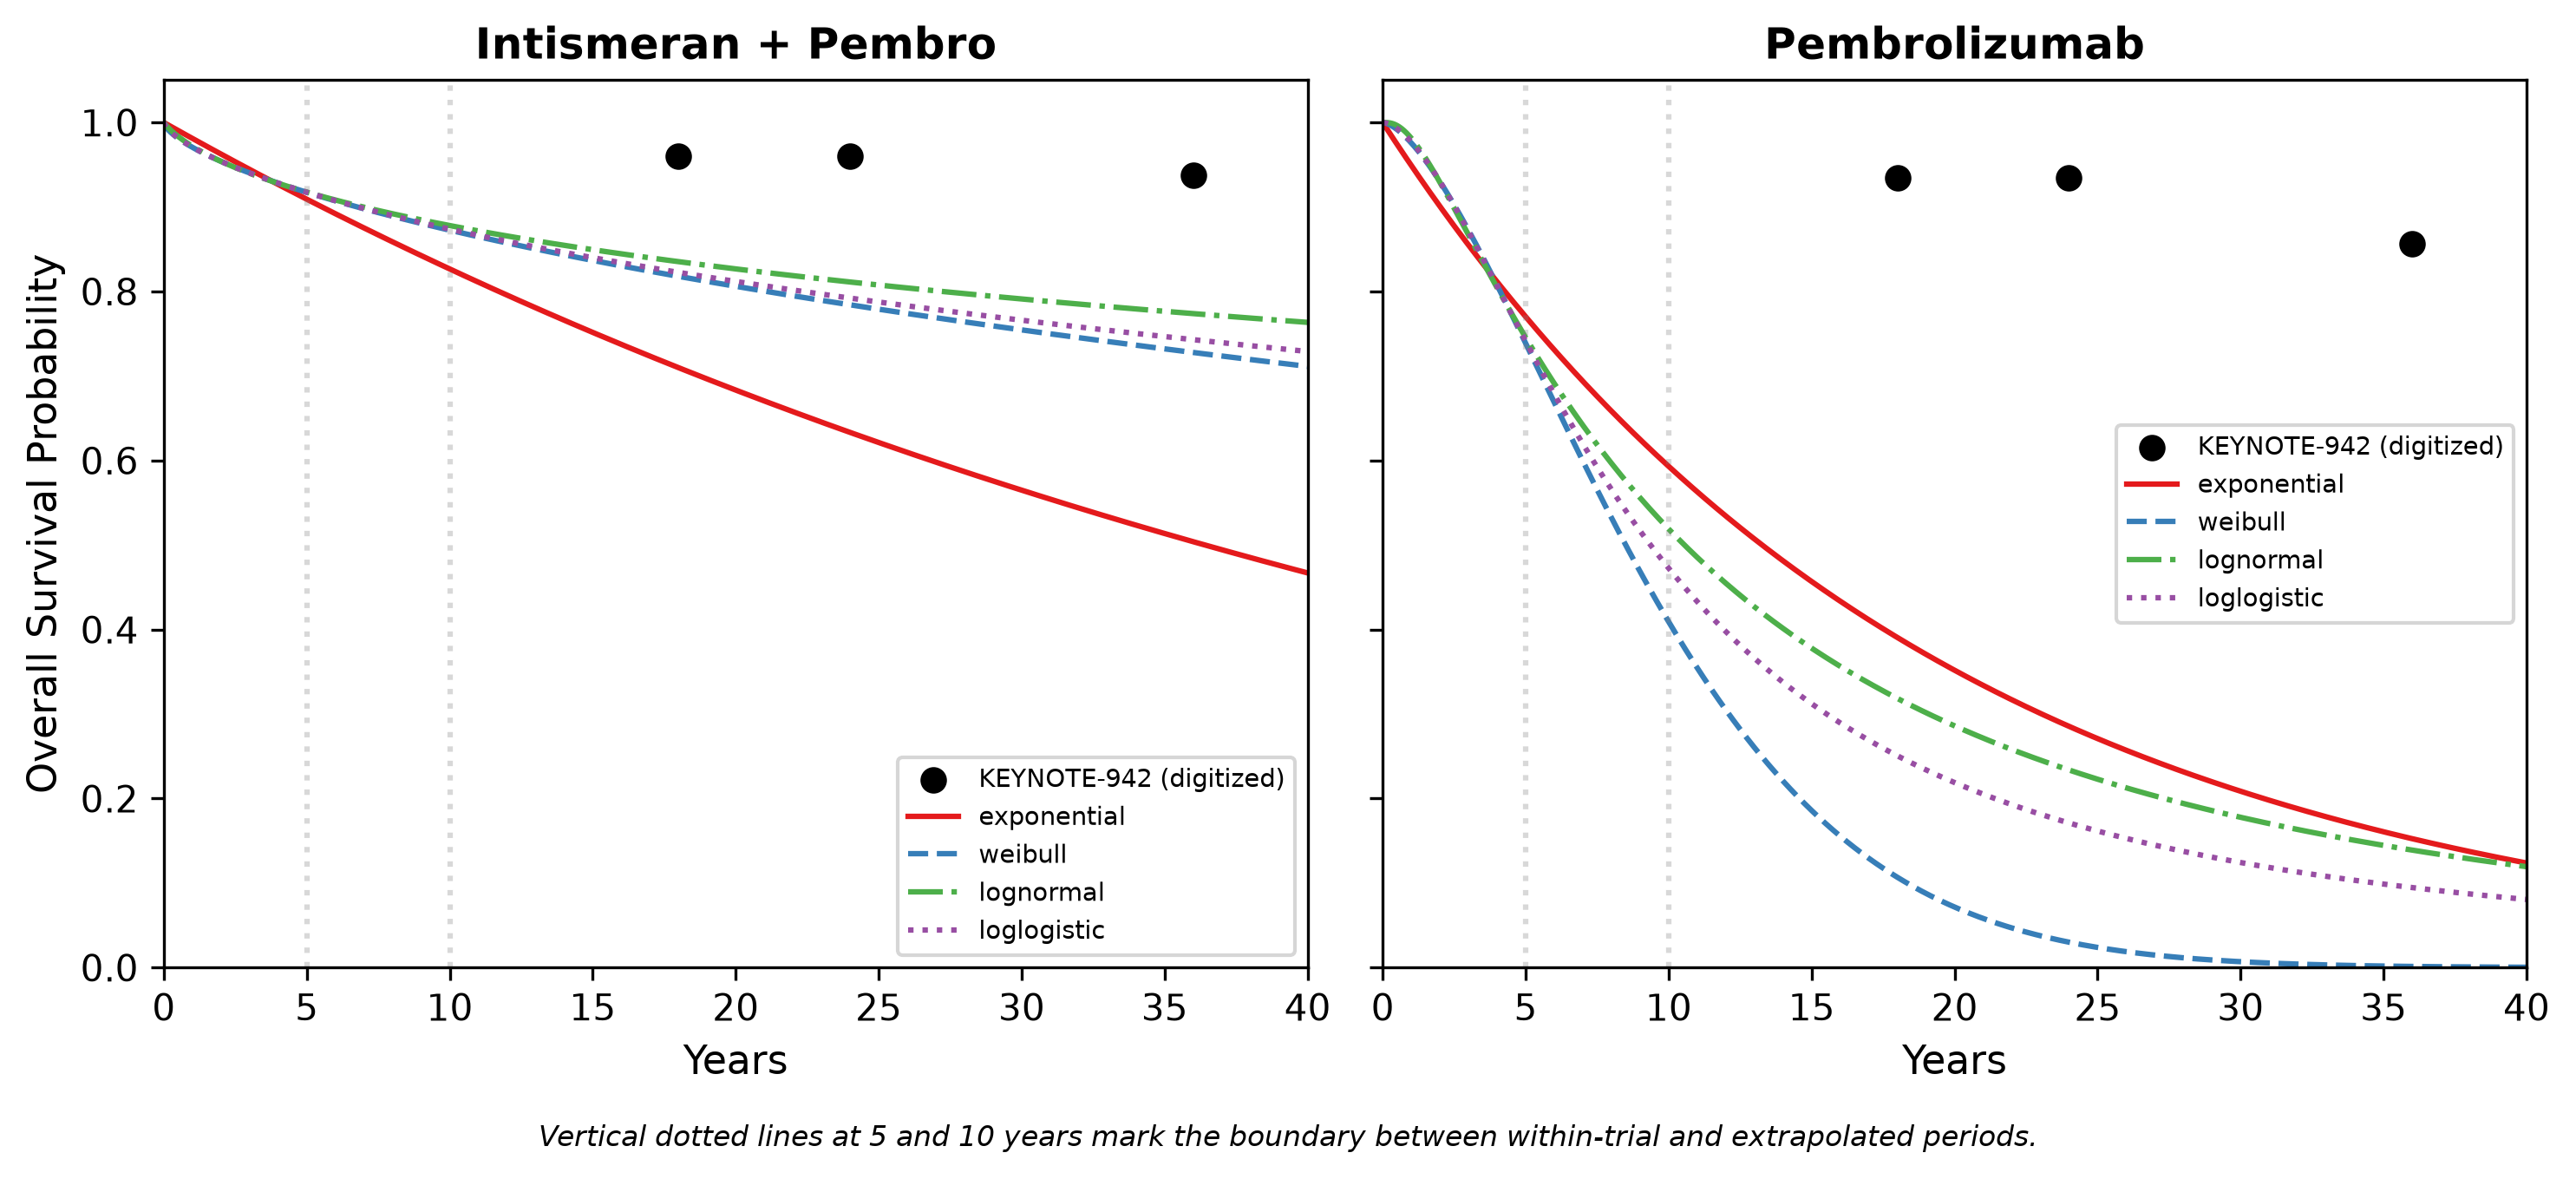
\includegraphics[width=\textwidth]{fig_s3_os_extrapolation.png}
\caption{Lifetime OS extrapolation by parametric distribution. Within-trial data (0--5 years) are shown to the left of the first vertical dotted line; beyond 10 years is pure extrapolation. The four distributions produce wildly divergent 40-year survival estimates (0\% to 76.3\%).}
\label{fig:s3}
\end{figure}

% ═══════════════════════════════════════════════════
\section{General-Population Mortality and Structural Validation}
% ═══════════════════════════════════════════════════

\subsection{GP Mortality Implementation}
\label{sec:gp_impl}
The GP mortality hazard floor is applied to modeled OS from month 60 onward.

\textbf{Life table source:} US 2019 period life tables (Arias et al., NVSS).
\textbf{Baseline age:} 61 years (KEYNOTE-942 median). \textbf{Sex weighting:} 64\% male, 36\% female.
\textbf{Interpolation:} Annual life table survival linearly interpolated to monthly resolution; monthly hazards derived as $h_{\text{GP}}(t) = -\ln[S_{\text{GP}}(t{+}1)/S_{\text{GP}}(t)]$.
\textbf{Constraint formula (mortality hazard floor):} from month 60 onward, the model mortality hazard is floored at the age- and sex-matched general-population hazard:
\begin{equation}
    h_{\text{model}}^{\text{con}}(t) = \max\left[h_{\text{param}}(t),\; h_{\text{GP}}(t)\right] \qquad t \geq 60 \text{ months},
\end{equation}
where $h_{\text{param}}(t) = -\ln[S_{\text{param}}(t{+}1)/S_{\text{param}}(t)]$ is the monthly hazard implied by the fitted parametric survival curve. The constrained survival is reconstructed as $S_{\text{model}}^{\text{con}}(t) = \exp[-\sum_{0}^{t} h^{\text{con}}(u)]$. This is a \textbf{hazard floor}, not a survival cap: a cohort that has already experienced elevated (cancer-related) mortality in the first 5 years remains below general-population survival at every subsequent time point, whereas a survival cap ($S = \min[S_{\text{param}}, S_{\text{GP}}]$) would incorrectly force the two curves to coincide whenever the parametric tail exceeded the general-population level. Both arms are subject to the same background mortality floor.

\subsection{Long-Term Survival Diagnostics}
\label{sec:longterm}
\begin{table}[H]
\centering
\caption{Long-Term Survival Predictions vs.\ General Population}
\label{tab:s5}
\begin{tabular}{lcccc}
\toprule
\textbf{Year} & \textbf{Combo OS} & \textbf{Pembro OS} & \textbf{GP Survival} & \textbf{Combo vs GP} \\
\midrule
5 & 91.6\% & 74.1\% & 93.3\% & Below (excess mortality to date) \\
10 & 82.5\% & 51.6\% & 84.1\% & Below (hazard floor active) \\
15 & 70.8\% & 37.6\% & 72.2\% & Below (hazard floor active) \\
20 & 56.1\% & 28.4\% & 57.3\% & Below (hazard floor active) \\
30 & 21.5\% & 10.9\% & 22.1\% & Below (hazard floor active) \\
40 & 0.0\% & 0.0\% & 0.0\% & At GP (age 101, GP survival $\approx$ 0) \\
\bottomrule
\end{tabular}
\end{table}

\subsection{OS versus General-Population Survival}
\label{sec:os_vs_gp}
\begin{figure}[H]
\centering
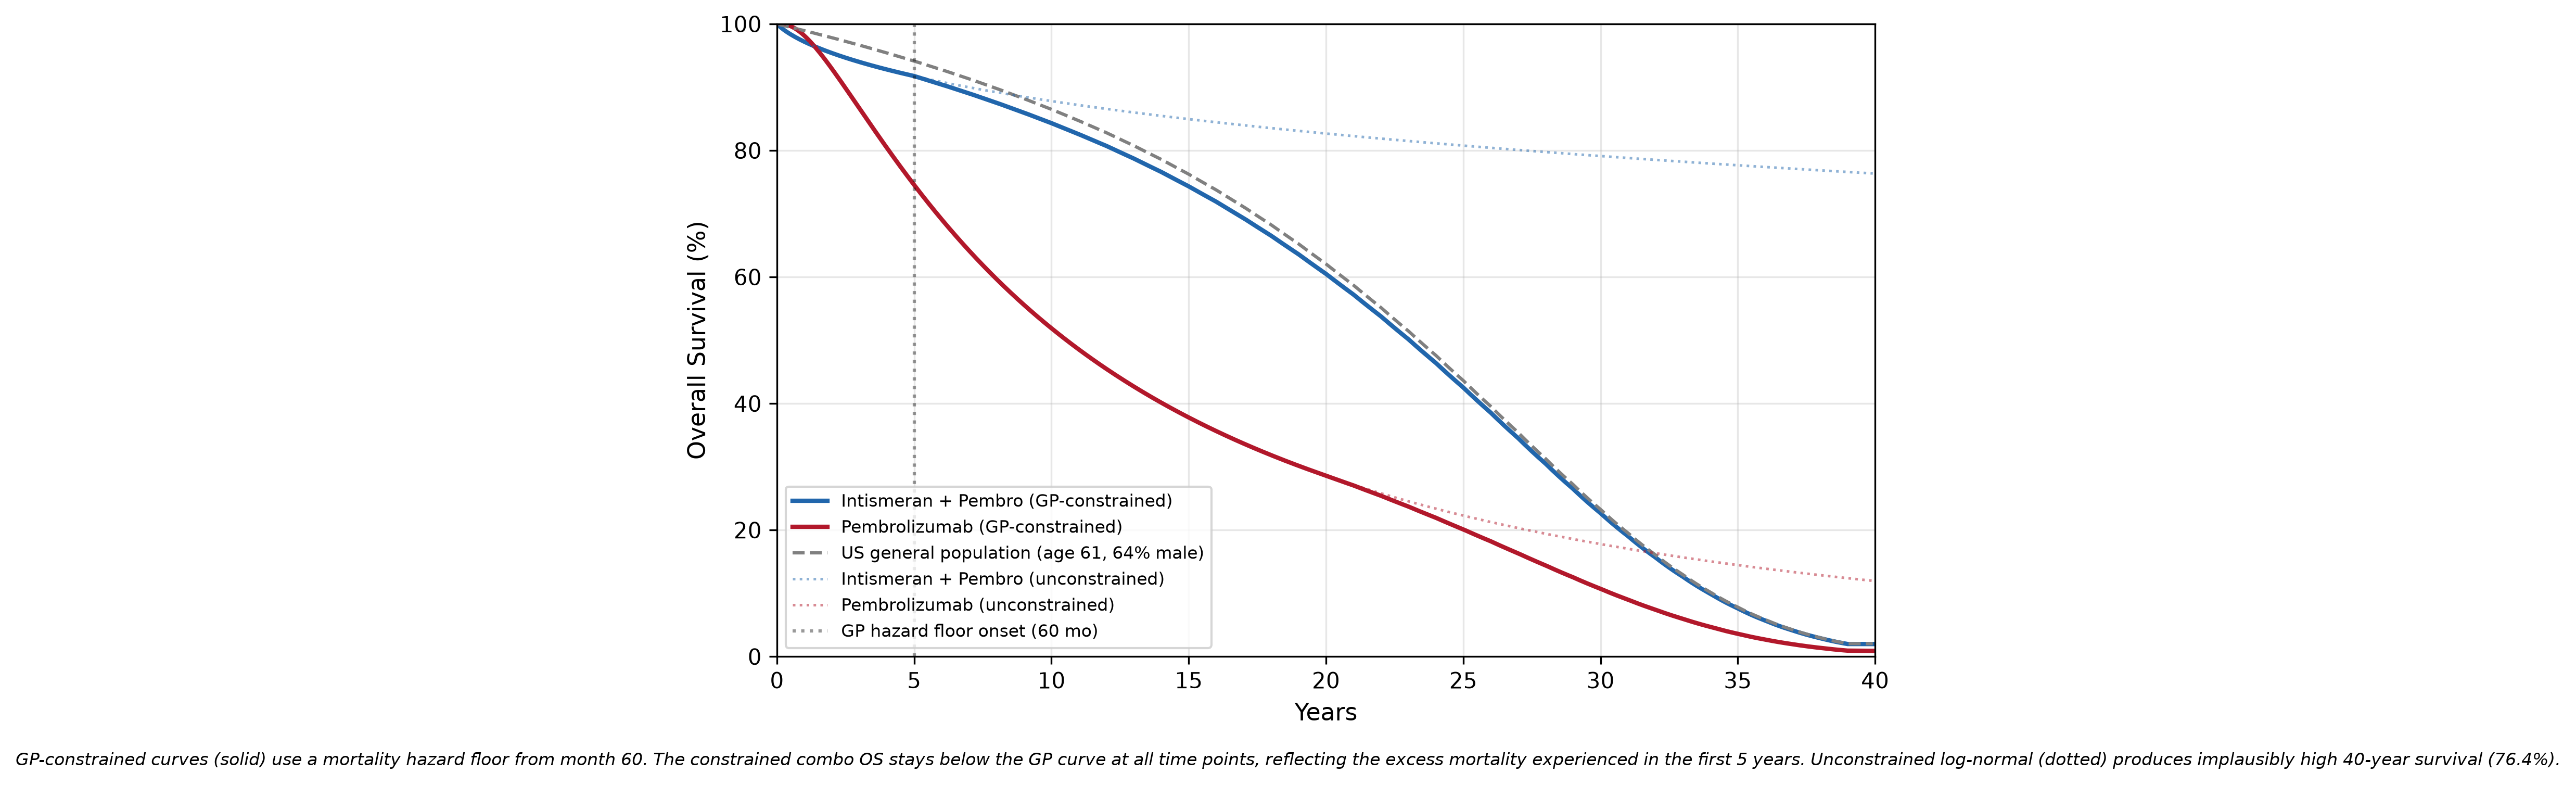
\includegraphics[width=\textwidth]{fig_s4_os_vs_gp.png}
\caption{OS versus general population. Solid lines: GP-constrained model (hazard floor from 60 months). Dotted lines: unconstrained log-normal extrapolation. Dashed gray line: US GP survival from age 61. The constrained combo curve remains below the GP curve at all time points, reflecting the hazard-floor property: a cohort with prior excess mortality does not "catch up" to general-population survival.}
\label{fig:s4}
\end{figure}

\subsection{Structural Quality Assurance}
\label{sec:structural_qa}
\begin{table}[H]
\centering
\caption{Structural Quality Assurance (480 Monthly Cycles)}
\label{tab:s6}
\begin{tabular}{lc}
\toprule
\textbf{Check} & \textbf{Result} \\
\midrule
Total cycles & 480 \\
RFS $>$ DMFS violations & 0 \\
DMFS $>$ OS violations & 0 \\
Negative RF state probability & 0 \\
Negative LR state probability & 0 \\
Negative DM state probability & 0 \\
Maximum state-sum error & $< 10^{-12}$ \\
Clamp events (forced non-negative) & 0 \\
\bottomrule
\end{tabular}
\end{table}

% ═══════════════════════════════════════════════════
\section{External Validation}
% ═══════════════════════════════════════════════════

\subsection{External Validation Landmarks}
\label{sec:external_landmarks}
\begin{table}[H]
\centering
\caption{External Validation of Pembrolizumab Arm Predictions}
\label{tab:s7}
\begin{tabular}{lcccc}
\toprule
\textbf{Outcome} & \textbf{Year} & \textbf{Model (pembro)} & \textbf{KEYNOTE-054} & \textbf{CheckMate 238} \\
\midrule
RFS & 5 & 40.5\% & --- & 51\% \cite{ascierto2025} \\
RFS & 7 & 31.9\% & 50\% \cite{eggermont2025} & 46\% \cite{ascierto2025} \\
DMFS & 5 & 53.8\% & --- & 59\% \cite{ascierto2025} \\
DMFS & 7 & 44.9\% & 54\% \cite{eggermont2025} & 55\% \cite{ascierto2025} \\
OS & 5 & 74.5\% & NR & 76\% \cite{ascierto2023} \\
OS & 7 & 64.2\% & NR & 71\% \cite{ascierto2025} \\
\bottomrule
\end{tabular}
\end{table}
\noindent\textit{NR: Not reported.} CheckMate 238 evaluated nivolumab (not pembrolizumab). The model predicts lower RFS/DMFS versus external trials, reflecting the higher-risk KEYNOTE-942 population (stage IIIB--IV including resected stage IV melanoma vs IIIA--C in KEYNOTE-054 and IIIB--IV in CheckMate 238). Only published landmark values are included; no extrapolated estimates are used.\cite{eggermont2025, ascierto2025}

\subsection{Longitudinal External Validation}
\label{sec:external_fig}
\begin{figure}[H]
\centering
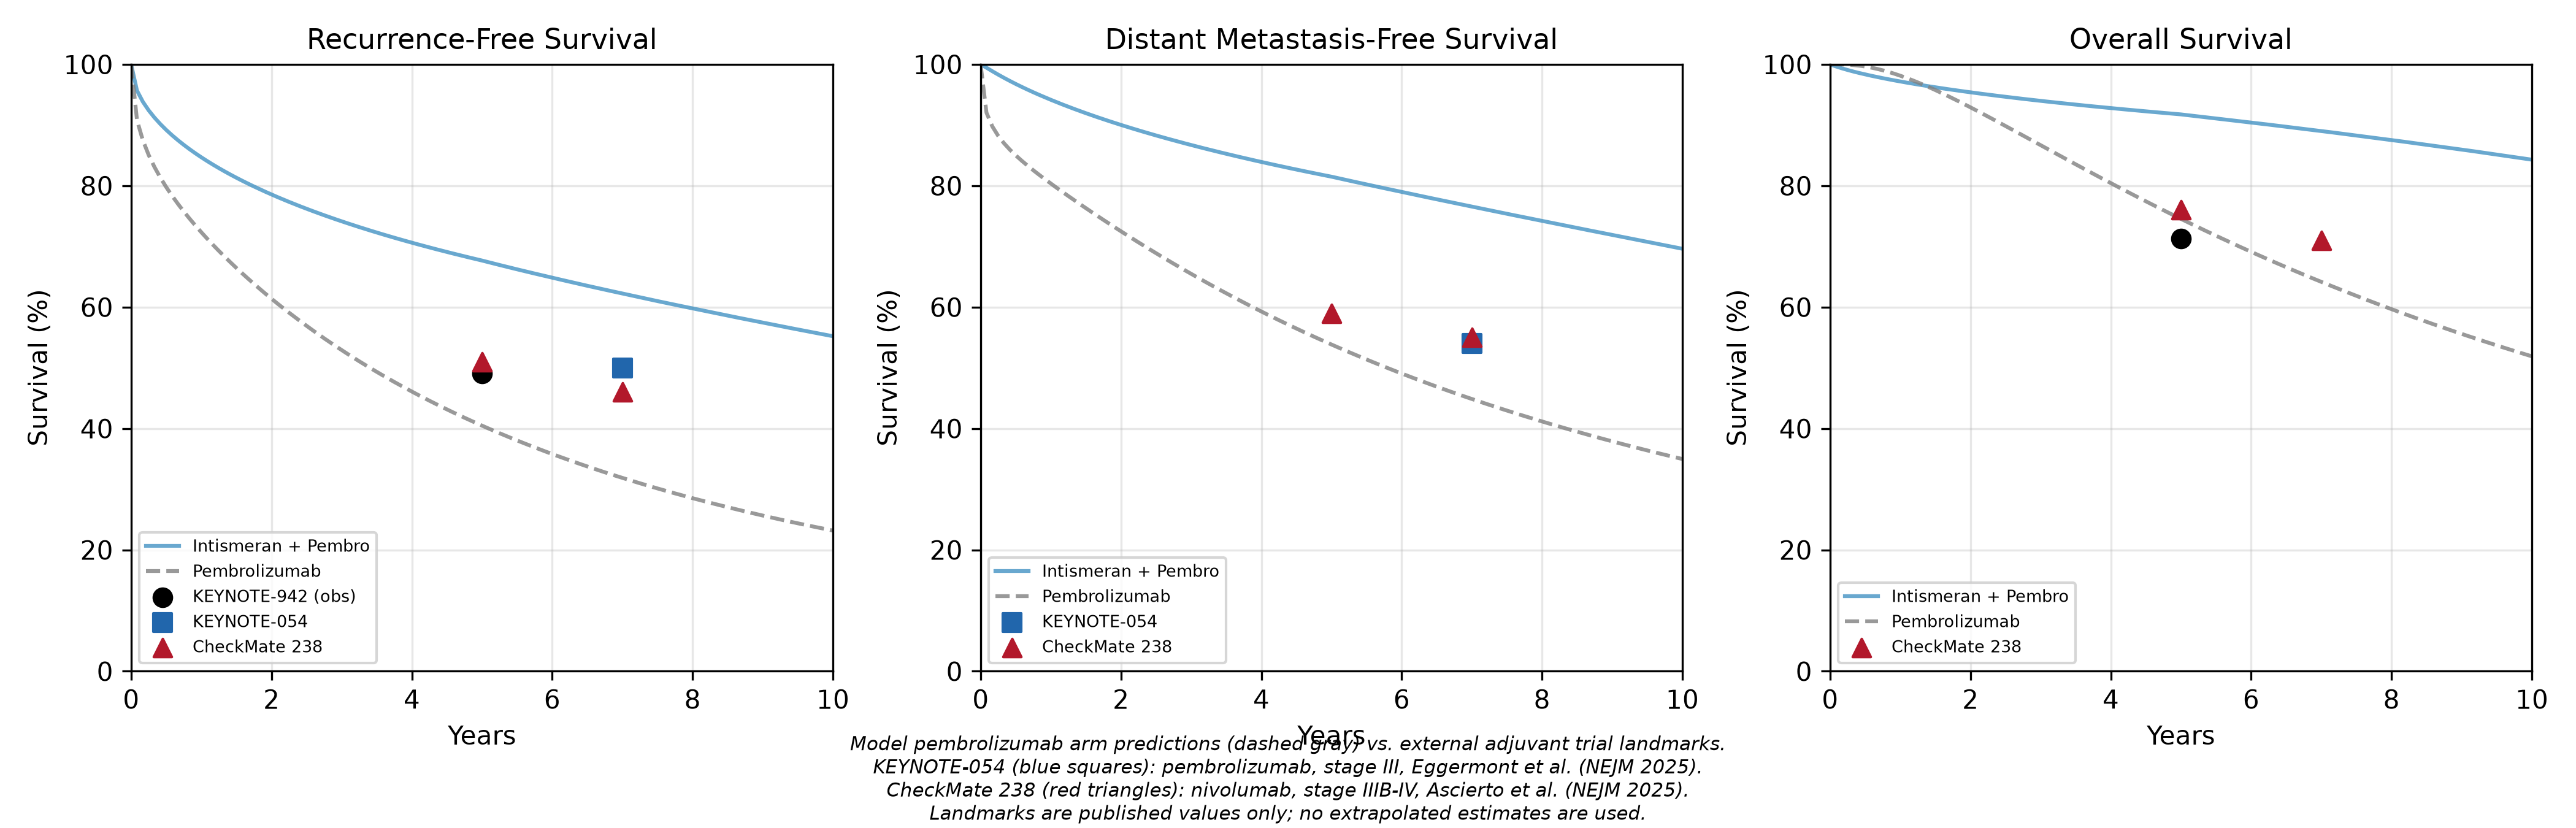
\includegraphics[width=\textwidth]{fig_s5_external_validation.png}
\caption{External validation of pembrolizumab arm predictions. Gray line: model. Circles: KEYNOTE-942 observed data. Squares: KEYNOTE-054 (pembrolizumab, 7-year). Triangles: CheckMate 238 (nivolumab, 5- and 7-year). Only published landmark values are shown.}
\label{fig:s5}
\end{figure}

% ═══════════════════════════════════════════════════
\section{Model Inputs}
% ═══════════════════════════════════════════════════
\label{sec:inputs}

\subsection{Complete Parameter Table}
\begin{landscape}
\begin{table}[p]
\centering
\caption{Full Model Parameter Inventory}
\label{tab:s8}
\footnotesize
\setlength{\tabcolsep}{4pt}
\renewcommand{\arraystretch}{0.95}
\begin{tabularx}{\linewidth}{@{}>{\raggedright\arraybackslash}Xlll>{\raggedright\arraybackslash}Xl@{}}
\toprule
\textbf{Parameter} & \textbf{Base} & \textbf{DSA Low} & \textbf{DSA High} & \textbf{PSA Distribution} & \textbf{Source} \\
\midrule
\multicolumn{6}{c}{\textit{Clinical Parameters}} \\
OS $\mu$ -- combo & 8.268 & 4.228 & 4.628 & Normal (SE from Jacobian) & Fitted \\
OS $\sigma$ -- combo & 0.478 & 0.378 & 0.578 & Normal (SE from Jacobian) & Fitted \\
OS $\mu$ -- pembro & 3.725 & 3.525 & 3.925 & Normal (SE from Jacobian) & Fitted \\
OS $\sigma$ -- pembro & 0.574 & 0.474 & 0.674 & Normal (SE from Jacobian) & Fitted \\
r$_{\text{DM}}$ $\mu$ -- combo & 4.107 & 3.907 & 4.307 & Normal (SE from Jacobian) & Fitted \\
r$_{\text{DM}}$ $\sigma$ -- combo & 0.432 & 0.332 & 0.532 & Normal (SE from Jacobian) & Fitted \\
r$_{\text{DM}}$ $\mu$ -- pembro & 2.849 & 2.649 & 3.049 & Normal (SE from Jacobian) & Fitted \\
r$_{\text{DM}}$ $\sigma$ -- pembro & 0.934 & 0.834 & 1.034 & Normal (SE from Jacobian) & Fitted \\
r$_{\text{LR}}$ $\mu$ -- combo & 3.367 & 3.167 & 3.567 & Normal (SE from Jacobian) & Fitted \\
r$_{\text{LR}}$ $\sigma$ -- combo & 0.624 & 0.524 & 0.724 & Normal (SE from Jacobian) & Fitted \\
r$_{\text{LR}}$ $\mu$ -- pembro & 2.750 & 2.550 & 2.950 & Normal (SE from Jacobian) & Fitted \\
r$_{\text{LR}}$ $\sigma$ -- pembro & 0.638 & 0.538 & 0.738 & Normal (SE from Jacobian) & Fitted \\
Treatment duration (pembro) & 18 cycles (2 yr) & 9 & 24 & Fixed & \cite{khattak2026} \\
Treatment duration (intismeran) & 9 doses (1 yr) & 6 & 12 & Fixed & \cite{khattak2026} \\
Baseline age & 61 years & 55 & 67 & Fixed & \cite{khattak2026} \\
Male proportion & 64\% & -- & -- & Fixed & \cite{khattak2026} \\
\midrule
\multicolumn{6}{c}{\textit{Costs (2026 USD)}} \\
Intismeran (one-time) & \$200,000 & \$160,000 & \$240,000 & Gamma (CV=0.2) & Assumed \\
Pembrolizumab (annual) & \$220,896 & \$176,717 & \$265,075 & Gamma (CV=0.2) & WAC (CMS) \\
Tumor sequencing & \$1,000 & \$500 & \$2,000 & Gamma (CV=0.2) & CMS \\
Administration (per cycle) & \$500 & \$250 & \$750 & Gamma (CV=0.2) & CMS \\
AE management (one-time) & \$15,000 & \$7,500 & \$22,500 & Gamma (CV=0.2) & \cite{zhang2023} \\
LR management (monthly) & \$3,000 & \$2,400 & \$3,600 & Gamma (CV=0.2) & \cite{zhang2023} \\
DM management (monthly) & \$12,000 & \$9,600 & \$14,400 & Gamma (CV=0.2) & \cite{bensimon2019} \\
\midrule
\multicolumn{6}{c}{\textit{Utilities}} \\
RF state & 0.83 & 0.80 & 0.86 & Beta (SE=0.03) & \cite{johnston2021} \\
LR state & 0.64 & 0.61 & 0.67 & Beta (SE=0.03) & \cite{johnston2021} \\
DM state & 0.55 & 0.52 & 0.58 & Beta (SE=0.03) & \cite{johnston2021} \\
AE disutility (one-time) & 0.05 & 0.00 & 0.10 & Beta (SE=0.02) & Assumed \\
\midrule
\multicolumn{6}{c}{\textit{Economic Parameters}} \\
Discount rate (costs, effects) & 3\% & 0\% & 5\% & Fixed (DSA only) & \cite{sanders2016} \\
Time horizon & 40 years & 10 & 20 & Fixed (scenario) & Assumed \\
Willingness-to-pay threshold & \$100K--\$150K/QALY & \$50K & \$200K & Fixed (scenario) & \cite{neumann2014} \\
Cost base year & 2026 USD & -- & -- & -- & Assumed \\
GP mortality source & US 2019 Life Tables & -- & -- & -- & NVSS (Arias 2022) \\
\bottomrule
\end{tabularx}
\end{table}
\end{landscape}

% ═══════════════════════════════════════════════════
\section{Additional Results}
% ═══════════════════════════════════════════════════

\subsection{Lifetime Cost Decomposition}
\label{sec:cost_decomp}
\begin{table}[H]
\centering
\caption{Lifetime Cost Decomposition by Component}
\label{tab:s9}
\begin{tabular}{lccc}
\toprule
\textbf{Component} & \textbf{Combo} & \textbf{Pembro} & \textbf{Incremental} \\
\midrule
Intismeran & \$200,000 & \$0 & \$200,000 \\
Pembrolizumab & \$217,888 & \$217,888 & \$0 \\
Sequencing & \$1,000 & \$0 & \$1,000 \\
Administration & \$493 & \$493 & \$0 \\
Adverse events & \$15,000 & \$0 & \$15,000 \\
LR management & \$112,203 & \$74,477 & \$37,726 \\
DM management & \$524,121 & \$453,082 & -\$71,039 \\
\midrule
\textbf{Total} & \textbf{\$1,070,705} & \textbf{\$745,939} & \textbf{\$324,765} \\
\bottomrule
\end{tabular}
\end{table}
\noindent The upfront \$200,000 intismeran cost is partially offset by \$71,039 in lower DM management costs, reflecting the DMFS HR of 0.411.

\subsection{LY and QALY Decomposition}
\label{sec:qaly_decomp}
\begin{table}[H]
\centering
\caption{Life-Year and QALY Decomposition by Health State}
\label{tab:s10}
\begin{tabular}{lccc}
\toprule
\textbf{Outcome} & \textbf{Combo} & \textbf{Pembro} & \textbf{Incremental} \\
\midrule
Life-years (undiscounted) & 23.78 & 15.34 & 7.13 \\
Life-years (discounted 3\%) & 19.01 & 10.75 & 8.26 \\
\midrule
RF state QALYs & 10.17 & 4.60 & 5.57 \\
LR state QALYs & 1.99 & 1.32 & 0.67 \\
DM state QALYs & 2.00 & 1.73 & -0.32 \\
\midrule
\textbf{Total QALYs} & \textbf{14.16} & \textbf{7.65} & \textbf{6.52} \\
\bottomrule
\end{tabular}
\end{table}
\noindent Health benefit is driven by RF state QALYs (5.57 gained), more than compensating for fewer DM-state QALYs (-0.32).

% ═══════════════════════════════════════════════════
\section{Uncertainty and Structural Scenario Analyses}
% ═══════════════════════════════════════════════════

\subsection{Deterministic Sensitivity Analysis}
\label{sec:dsa}
\begin{table}[H]
\centering
\caption{One-Way Deterministic Sensitivity Analysis}
\label{tab:s11}
\begin{tabular}{lrrrrr}
\toprule
\textbf{Parameter} & \textbf{Base} & \textbf{Low} & \textbf{High} & \textbf{ICER range} & \textbf{Change in NMB} \\
\midrule
Utility RF & 0.83 & 0.80 & 0.86 & 40,601--37,715 & \$27,691 \\
Utility LR & 0.64 & 0.61 & 0.67 & 39,224--38,987 & \$2,283 \\
Utility DM & 0.55 & 0.52 & 0.58 & 38,926--39,285 & \$3,447 \\
Pembrolizumab annual cost & \$220,896 & 176,717 & 265,075 & 49,841--49,841 & \$0 \\
Intismeran cost & \$200,000 & 160,000 & 240,000 & 28,461--49,749 & \$80,000 \\
LR monthly cost & \$3,000 & 2,400 & 3,600 & 38,376--39,834 & \$5,478 \\
DM monthly cost & \$12,000 & 9,600 & 14,400 & 43,508--34,702 & \$33,094 \\
Discount rate & 3\% & 0\% & 5\% & 31,092--47,814 & \$257,766 \\
OS $\mu$ combo & 8.268 & 4.228 & 4.628 & DQY $<$ 0 at low & \$37,797 \\
OS $\mu$ pembro & 3.725 & 3.525 & 3.925 & 59,135--57,130 & \$30,496 \\
\bottomrule
\end{tabular}
\end{table}
\noindent The ICER remained below \$60,000/QALY across all tested ranges.

\subsection{Probabilistic Sensitivity Analysis}
\label{sec:psa}

\subsubsection{PSA Implementation Details}
PSA with 6,000 Monte Carlo iterations (seed = 42). Survival parameters ($\mu$, $\sigma$ for 6 curves) drawn jointly from bivariate normal via Jacobian covariance ($r > 0.95$). Costs: gamma (CV=0.2). Utilities: beta (SE=0.03). Structural constraints (RFS $\leq$ DMFS $\leq$ OS, monotonicity, survival within [0,1]) verified every cycle; all 6,000 draws were structurally valid (0 rejections). No iterations were excluded on the basis of the ICER value.

\begin{landscape}
\begin{table}[p]
\centering
\caption{PSA Parameter Distributions and Sampled Values}
\label{tab:s12}
\footnotesize
\setlength{\tabcolsep}{5pt}
\begin{tabularx}{\linewidth}{@{}>{\raggedright\arraybackslash}Xlllll@{}}
\toprule
\textbf{Parameter} & \textbf{Distribution} & \textbf{Fitted mean} & \textbf{SE} & \textbf{Correlation} & \textbf{Sampling} \\
\midrule
OS $\mu$ / $\sigma$ -- combo & Bivariate normal & 8.396 / 3.096 & 0.793 / 0.522 & 0.996 & Joint \\
OS $\mu$ / $\sigma$ -- pembro & Bivariate normal & 4.841 / 1.131 & 0.291 / 0.310 & 0.955 & Joint \\
r$_{\text{DM}}$ $\mu$ / $\sigma$ -- combo & Bivariate normal & 7.113 / 2.480 & 0.814 / 0.563 & 0.995 & Joint \\
r$_{\text{DM}}$ $\mu$ / $\sigma$ -- pembro & Bivariate normal & 7.042 / 5.000 & 2.278 / 3.130 & 0.995 & Joint \\
r$_{\text{LR}}$ $\mu$ / $\sigma$ -- combo & Bivariate normal & 8.874 / 5.000 & 2.039 / 1.928 & 0.997 & Joint \\
r$_{\text{LR}}$ $\mu$ / $\sigma$ -- pembro & Bivariate normal & 5.913 / 2.674 & 0.757 / 0.879 & 0.984 & Joint \\
Intismeran cost & Gamma (CV=0.2) & \$200,000 & --- & --- & Independent \\
Pembrolizumab annual cost & Gamma (CV=0.2) & \$220,896 & --- & --- & Independent \\
LR monthly cost & Gamma (CV=0.2) & \$3,000 & --- & --- & Independent \\
DM monthly cost & Gamma (CV=0.2) & \$12,000 & --- & --- & Independent \\
Utility RF / LR / DM & Beta (SE=0.03) & 0.83 / 0.64 / 0.55 & --- & --- & Independent \\
\bottomrule
\end{tabularx}
\end{table}
\end{landscape}

\newpage
\subsubsection{PSA Results}
\begin{itemize}
\item Mean $\Delta$QALY: 6.65 (95\% CI 4.13--9.83).
\item Mean $\Delta$Cost: \$293,238 (95\% CI \textendash\$533,282 to \$825,708).
\item Mean NMB: \$371,570 at \$100K and \$703,975 at \$150K.
\item Probability cost-effective: 52.4\% at \$50K, 93.4\% at \$100K, and 98.4\% at \$150K.
\item No iterations were excluded based on the ICER; 11.2\% of draws were cost-saving, and all 6,000 draws had $\Delta$QALY > 0.
\end{itemize}

\subsubsection{PSA Convergence}
\begin{figure}[H]
\centering
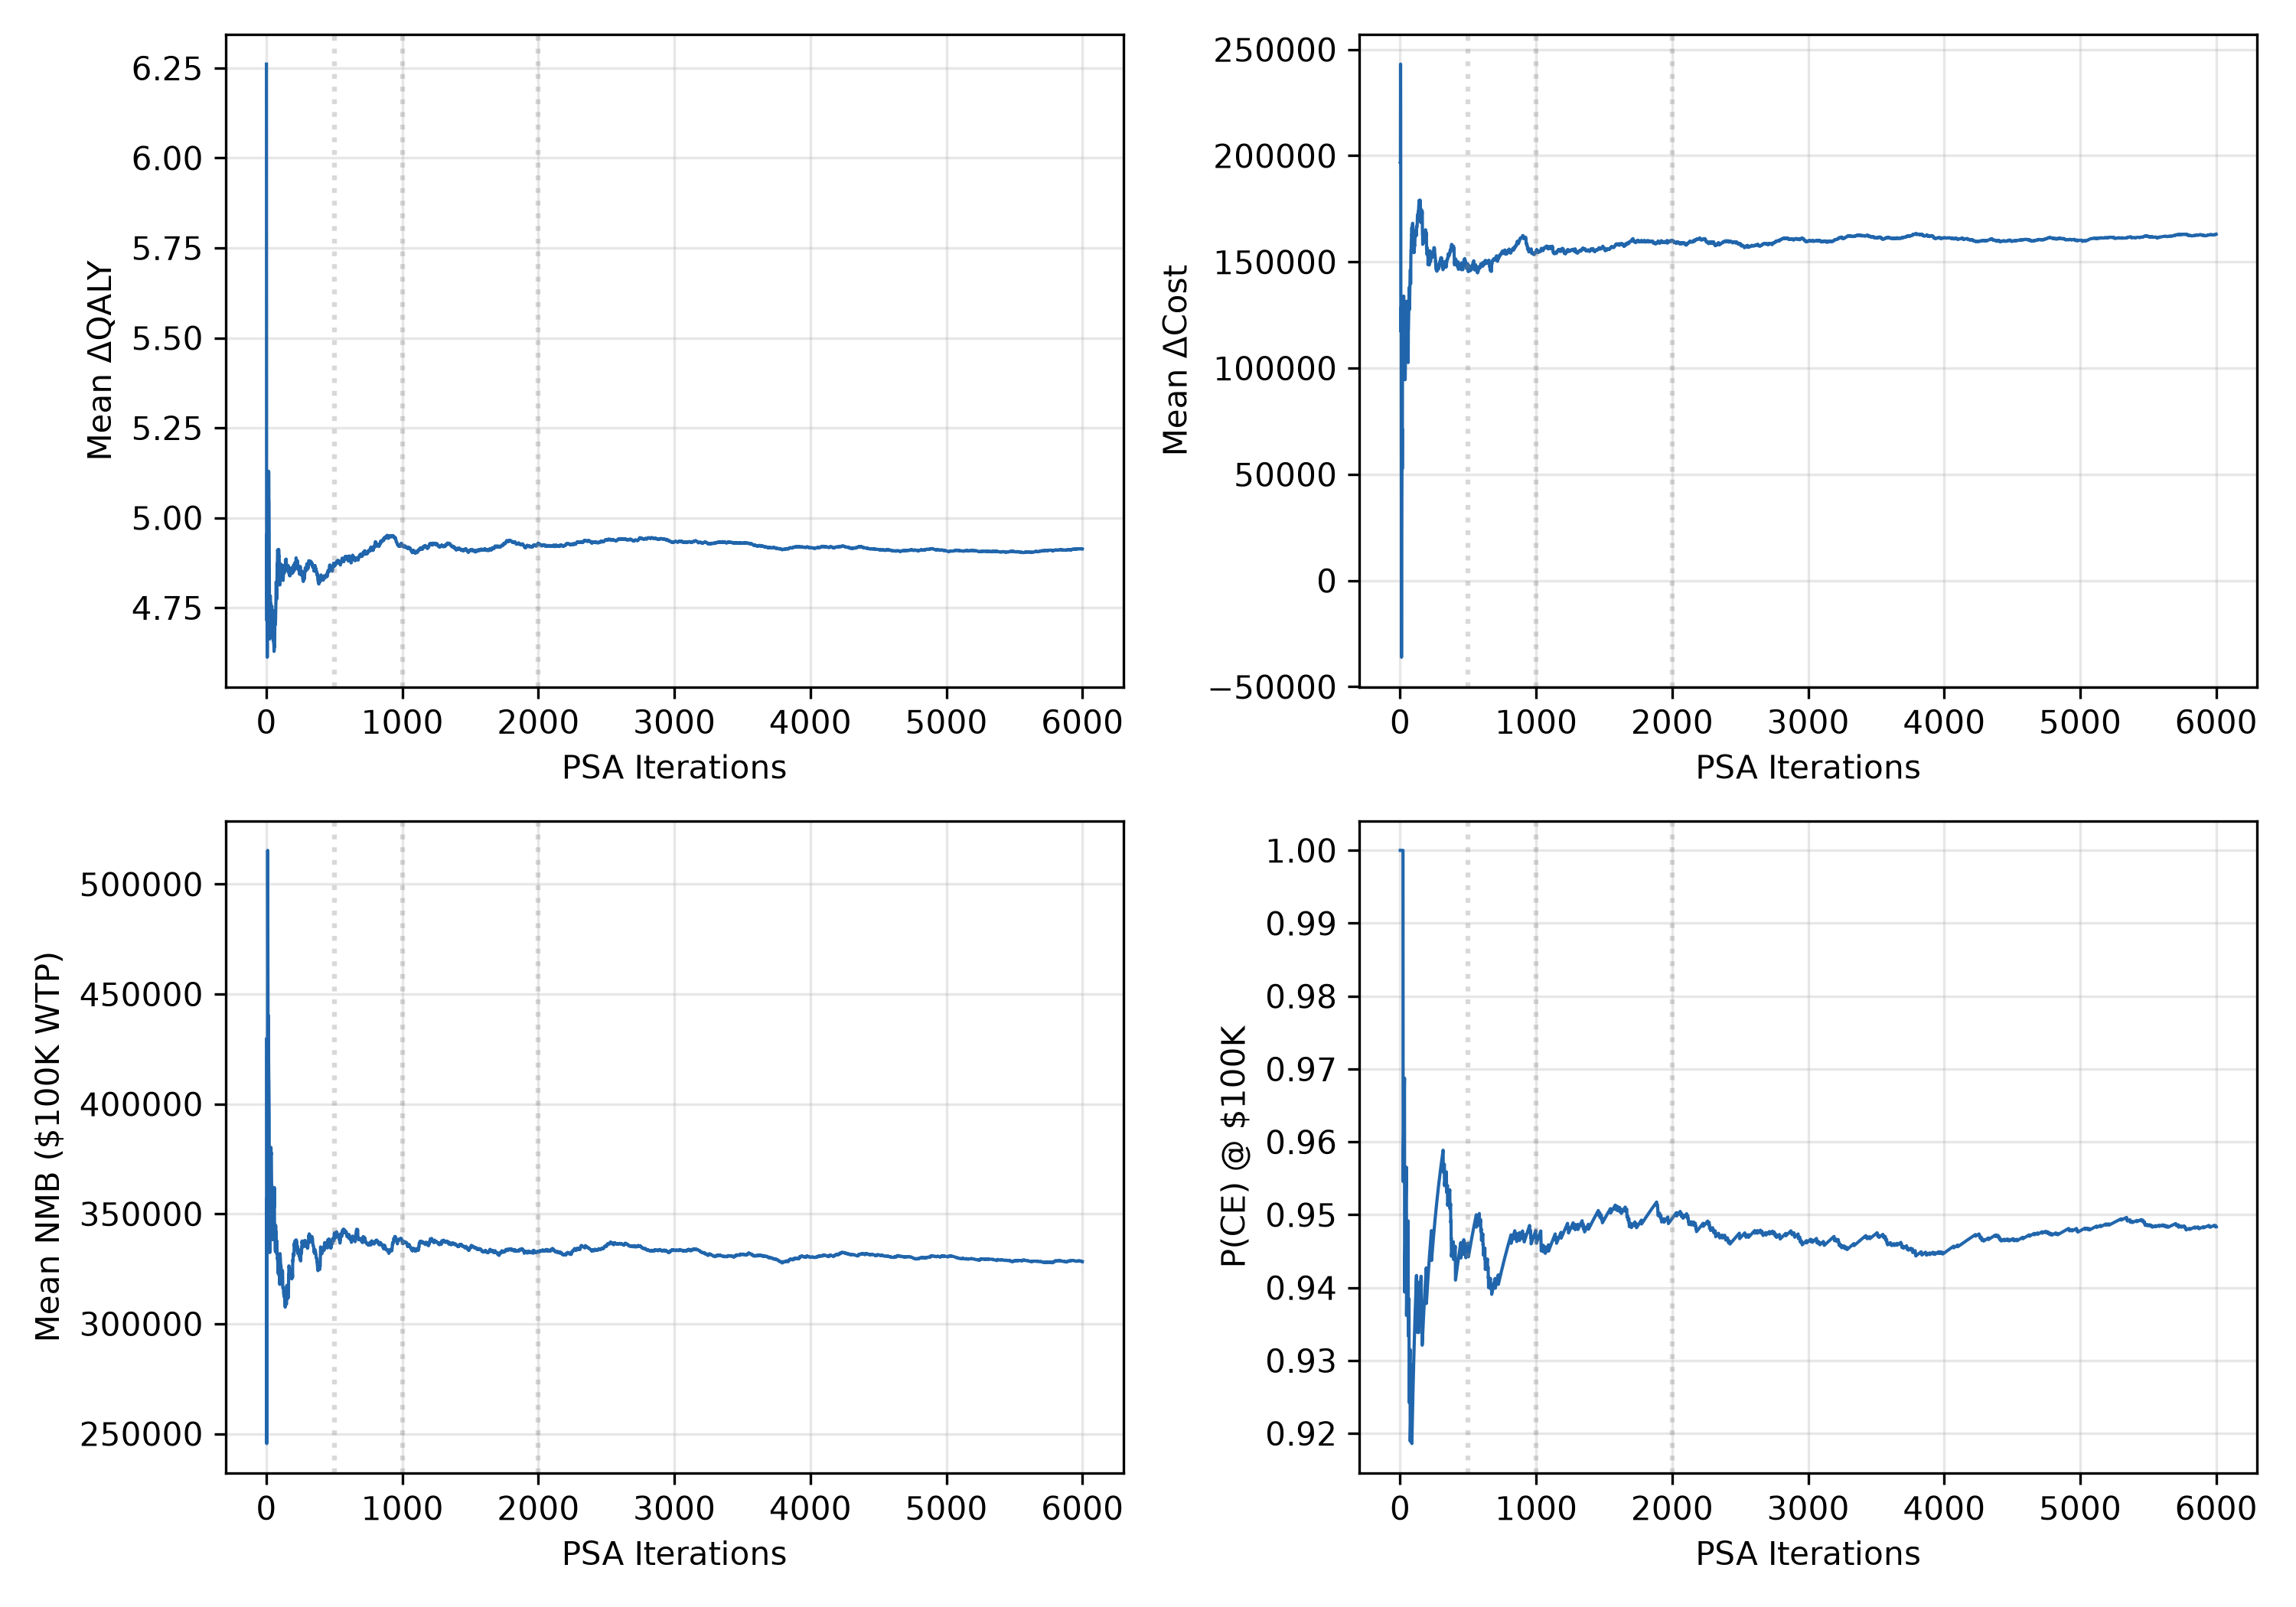
\includegraphics[width=\textwidth]{fig_s6_psa_convergence.png}
\caption{PSA convergence across iteration counts (6,000 structurally valid iterations, 0 structural rejections, seed = 42). Cumulative means of $\Delta$QALY, $\Delta$Cost, NMB, and P(CE). Vertical dotted lines at 500, 1,000, 2,000, and 4,000 iterations. Estimates stable from $\sim$500 iterations.}
\label{fig:s6}
\end{figure}

\subsubsection{Cost-Effectiveness Plane}
\begin{figure}[H]
\centering
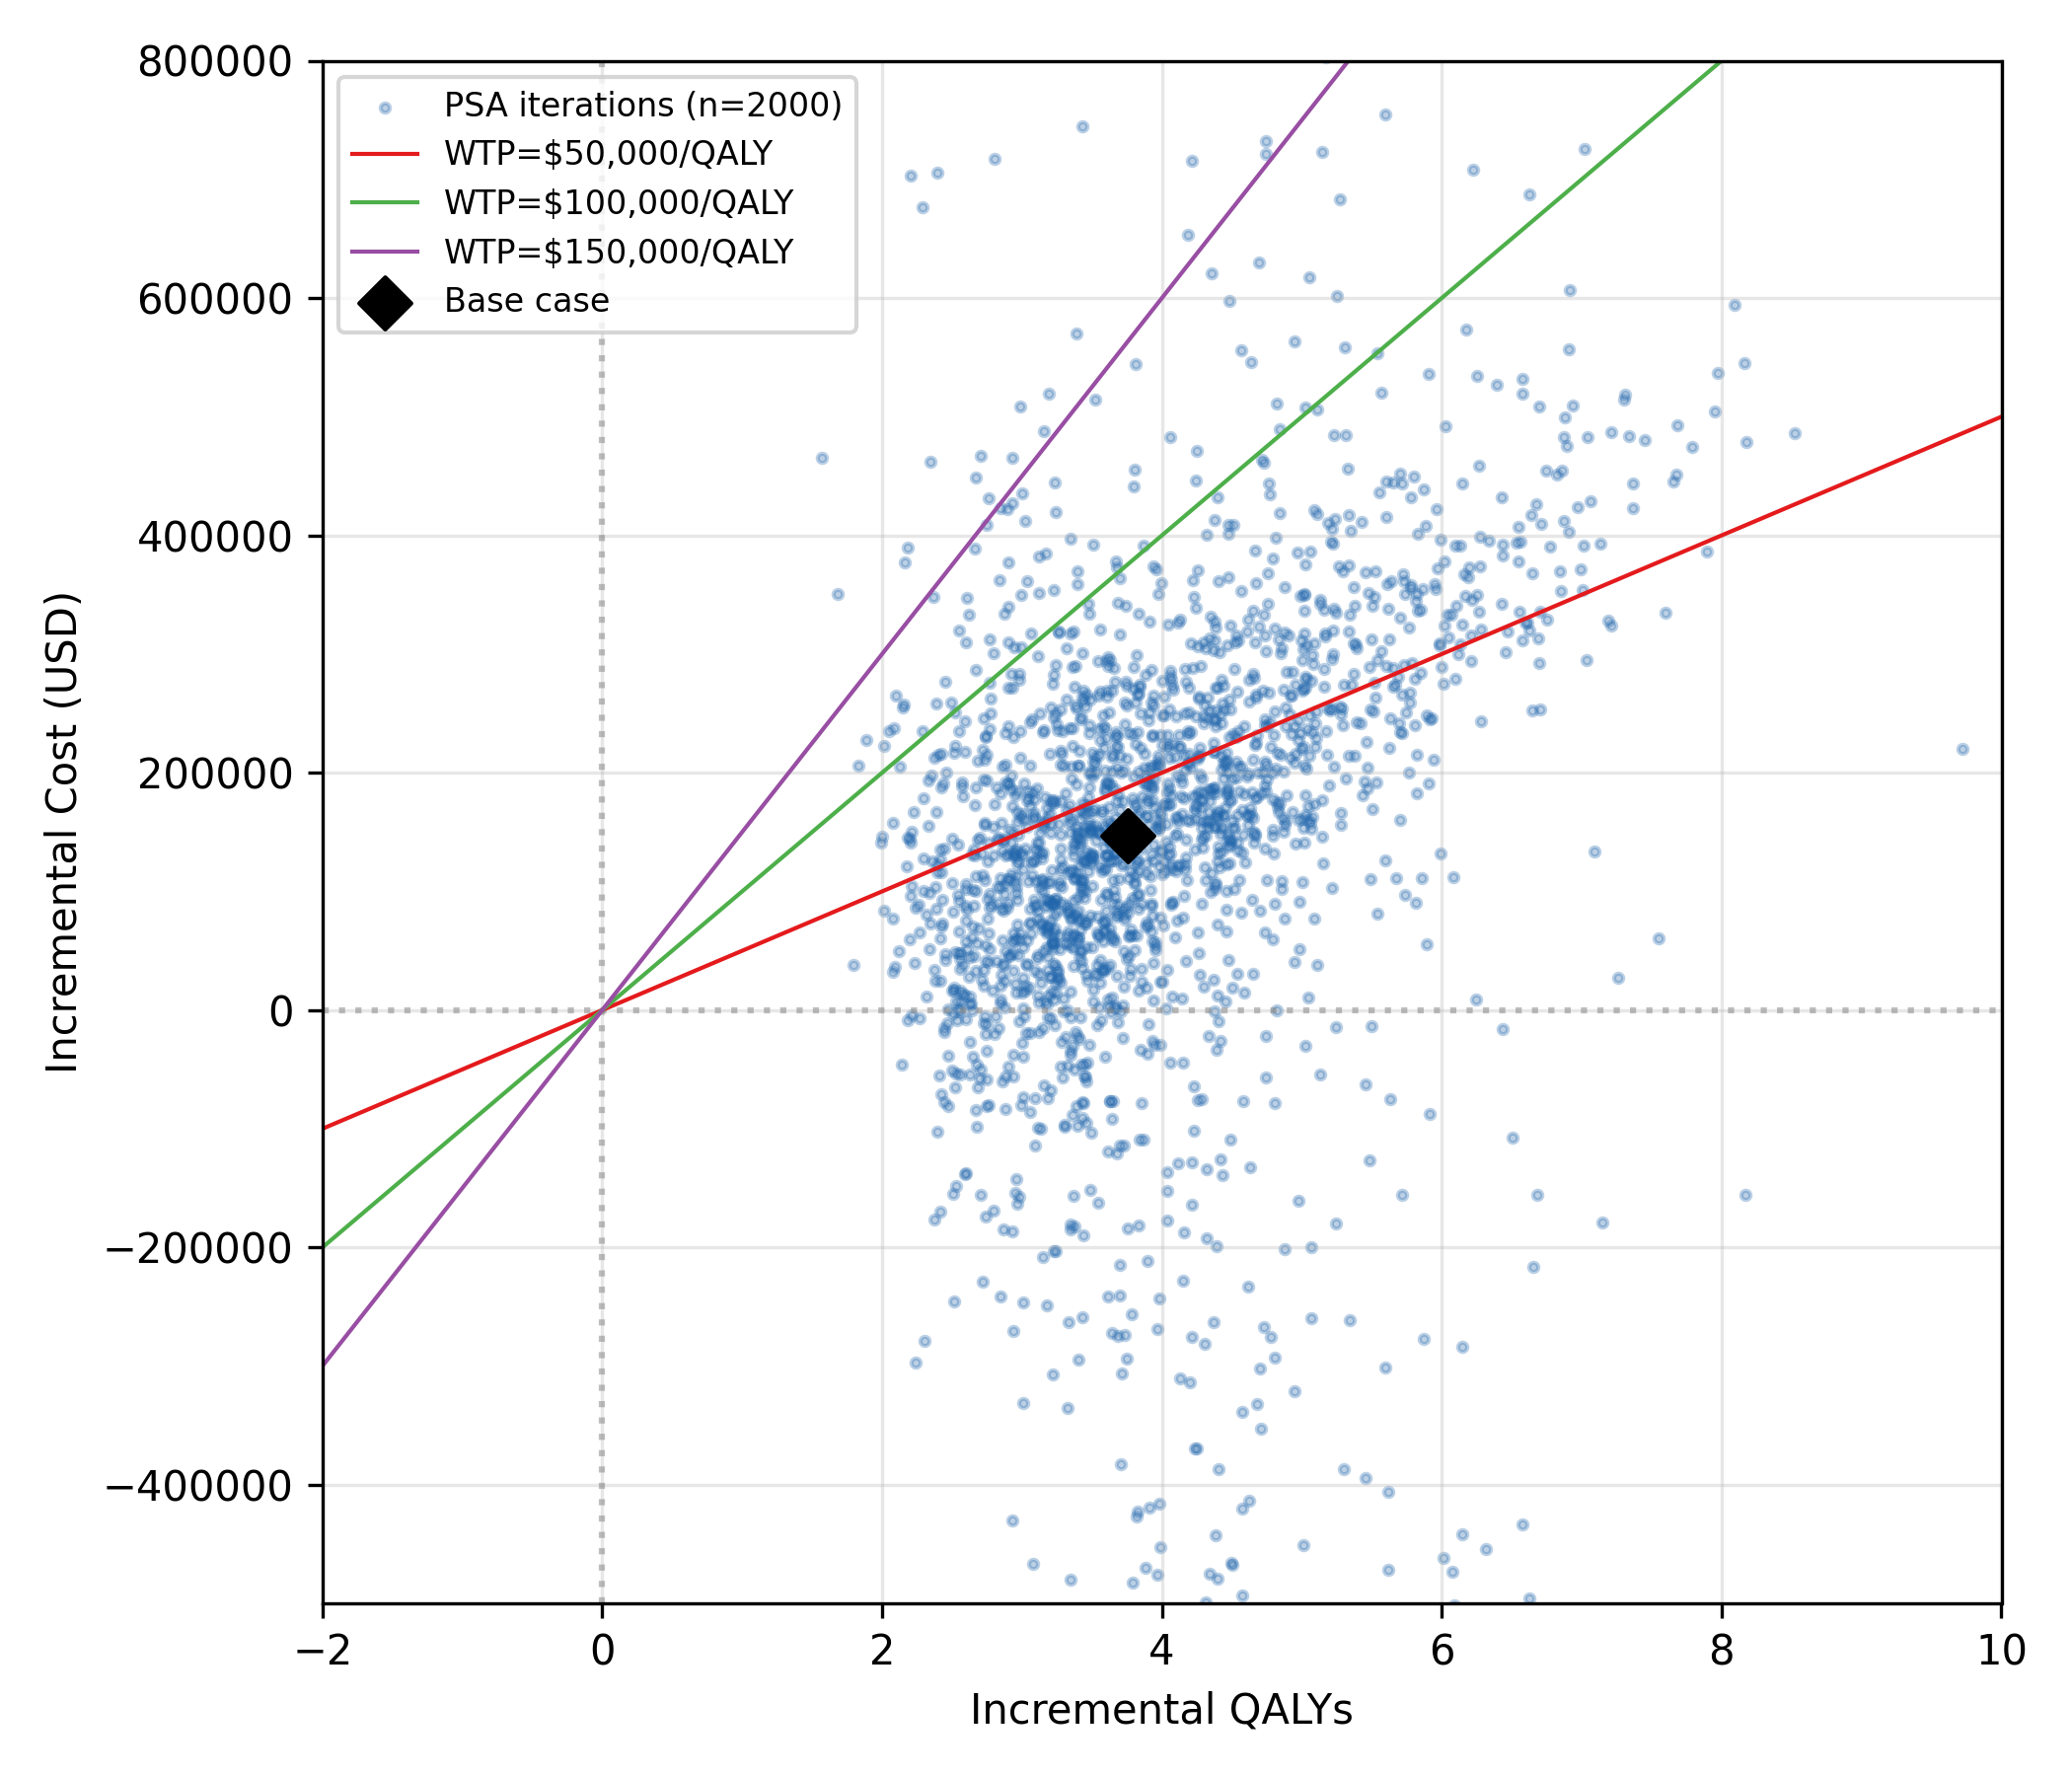
\includegraphics[width=\textwidth]{fig_s7_ce_plane.png}
\caption{CE plane showing 6,000 PSA iterations (blue), WTP lines (\$50K, \$100K, \$150K per QALY), and the deterministic base case (black diamond). 11.2\% of iterations fall in the southeast quadrant (cost-saving); all 6,000 iterations had positive $\Delta$QALY. No iterations were excluded based on the ICER value.}
\label{fig:s7}
\end{figure}

\subsection{Structural Scenario Analyses}
\label{sec:scenarios}
\begin{landscape}
\begin{table}[p]
\centering
\caption{Structural Scenario Analysis Results}
\label{tab:s13}
\footnotesize
\setlength{\tabcolsep}{5pt}
\begin{tabularx}{\linewidth}{@{}>{\raggedright\arraybackslash}Xrrrrrr@{}}
\toprule
\textbf{Scenario} & \textbf{$\Delta$LY} & \textbf{$\Delta$QALY} & \textbf{$\Delta$Cost} & \textbf{ICER} & \textbf{NMB \$100K} & \textbf{NMB \$150K} \\
\midrule
Base case & 8.26 & 6.52 & \$324,765 & \$49,841 & \$326,840 & \$652,643 \\
Weibull OS & 6.77 & 5.35 & \$293,679 & \$59,959 & \$241,047 & \$508,411 \\
Unconstrained (no GP) & 9.24 & 7.22 & \$373,488 & \$51,753 & \$348,189 & \$709,028 \\
GP floor 48 mo & 4.37 & 3.72 & \$145,054 & \$39,014 & \$226,750 & \$412,652 \\
GP floor 60 mo (base) & 8.26 & 6.52 & \$324,765 & \$49,841 & \$326,840 & \$652,643 \\
GP floor 72 mo & 4.50 & 3.81 & \$149,673 & \$39,251 & \$231,648 & \$422,309 \\
GP floor 96 mo & 4.69 & 3.96 & \$157,038 & \$39,696 & \$238,563 & \$436,363 \\
10-year horizon & 1.27 & 1.28 & \$95,573 & \$74,945 & \$31,951 & \$95,714 \\
20-year horizon & 3.32 & 2.91 & \$115,739 & \$41,785 & \$175,548 & \$321,191 \\
30-year horizon & 4.28 & 3.63 & \$140,823 & \$40,500 & \$222,152 & \$403,639 \\
40-year horizon (base) & 8.26 & 6.52 & \$324,765 & \$49,841 & \$326,840 & \$652,643 \\
Intismeran \$100K & 8.26 & 6.52 & \$46,961 & \$12,496 & \$328,851 & \$516,757 \\
Intismeran \$200K (base) & 8.26 & 6.52 & \$324,765 & \$49,841 & \$326,840 & \$652,643 \\
Intismeran \$300K & 8.26 & 6.52 & \$246,961 & \$65,714 & \$128,851 & \$316,757 \\
Intismeran \$500K & 8.26 & 6.52 & \$446,961 & \$118,932 & -\$71,149 & \$116,757 \\
Waning V1 (recurrence) & 1.83 & 1.87 & \$38,544 & \$20,591 & \$148,647 & \$242,242 \\
Waning V2 (hazard convergence) & 2.66 & 2.47 & \$74,620 & \$30,176 & \$172,659 & \$296,299 \\
No direct OS benefit & 0.00 & 0.50 & -\$14,562 & Dominant & \$64,131 & \$88,915 \\
\bottomrule
\end{tabularx}
\end{table}
\end{landscape}
\noindent The base-case conclusion is robust across structural assumptions. The ICER alone is insufficient: unconstrained model has moderate ICER (\$51,753) but implausible \$373,488 cost.

\noindent \textbf{Time horizon sensitivity.} The ICER was stable from the 20-year horizon onward: \$41,785 at 20 years, \$40,500 at 30 years, and \$49,841 at the 40-year base-case horizon (Table~\ref{tab:s13}). The difference between the 30- and 40-year ICER was \$308/QALY (0.8\%). Because the general-population mortality hazard floor was applied from 60 months onward and both costs and QALYs were discounted at 3\% annually, survival beyond the 20--30-year window contributed negligibly to discounted incremental costs and QALYs. This indicates that the 40-year lifetime horizon did not materially drive the base-case ICER, and that results were not sensitive to the choice of extrapolation window beyond approximately two decades.

\noindent \textbf{General population hazard floor start-time sensitivity.} The GP mortality floor was applied from 60 months in the base case. To assess whether the ICER was sensitive to the timing of floor application, we varied the start time from 48 to 96 months (Table~S14). The ICER ranged from \$39,014 (48-month floor) to \$39,696 (96-month floor), a spread of only \$682/QALY (1.7\%). This narrow range reflects the fact that the hazard floor does not materially affect the within-trial survival difference, which is already established by 48 months, and the floor's primary effect is to constrain the heavily discounted long-term extrapolation regardless of whether it begins at 48 or 96 months. The ICER is therefore robust to the exact timing of GP floor application.

% ═══════════════════════════════════════════════════
\section{Deterministic Threshold Acquisition Price}
% ═══════════════════════════════════════════════════

\subsection{Price Threshold Analysis}
\label{sec:price_threshold}
\begin{table}[H]
\centering
\caption{Price Threshold Analysis}
\label{tab:s14}
\begin{tabular}{lrrr}
\toprule
\textbf{Intismeran Price} & \textbf{ICER} & \textbf{NMB @ \$100K} & \textbf{NMB @ \$150K} \\
\midrule
\$0 & -\$14,113 & \$428,851 & \$616,757 \\
\$50,000 & -\$809 & \$378,851 & \$566,757 \\
\$100,000 & \$12,496 & \$328,851 & \$516,757 \\
\$150,000 & \$25,800 & \$278,851 & \$466,757 \\
\$200,000 (base) & \$49,841 & \$326,840 & \$652,643 \\
\$250,000 & \$52,409 & \$178,851 & \$366,757 \\
\$300,000 & \$65,714 & \$128,851 & \$316,757 \\
\$350,000 & \$79,019 & \$78,851 & \$266,757 \\
\$400,000 & \$92,323 & \$28,851 & \$216,757 \\
\textbf{\$527,344} & \textbf{\$100,077} & \textbf{-\$226} & \$187,680 \\
\$450,000 & \$105,628 & -\$21,149 & \$166,757 \\
\$500,000 & \$118,932 & -\$71,149 & \$116,757 \\
\$550,000 & \$132,237 & -\$121,149 & \$66,757 \\
\$600,000 & \$145,541 & -\$171,149 & \$16,757 \\
\textbf{\$852,051} & \textbf{\$149,909} & \textbf{-\$187,604} & \textbf{\$302} \\
\$650,000 & \$158,846 & -\$221,149 & -\$33,243 \\
\$700,000 & \$172,150 & -\$271,149 & -\$83,243 \\
\$750,000 & \$185,455 & -\$321,149 & -\$133,243 \\
\$800,000 & \$198,759 & -\$371,149 & -\$183,243 \\
\bottomrule
\end{tabular}
\end{table}
\noindent Deterministic threshold prices (from Table~\ref{tab:s14}): approximately \$527,000 at \$100,000/QALY (2.1$\times$ base) and approximately \$852,000 at \$150,000/QALY (3.1$\times$ base). These are model-based deterministic estimates; PSA uncertainty propagation and formal budget-impact analysis would be needed to inform payer negotiations.

\subsection{ICER versus Acquisition Price}
\label{sec:price_fig}
\begin{figure}[H]
\centering
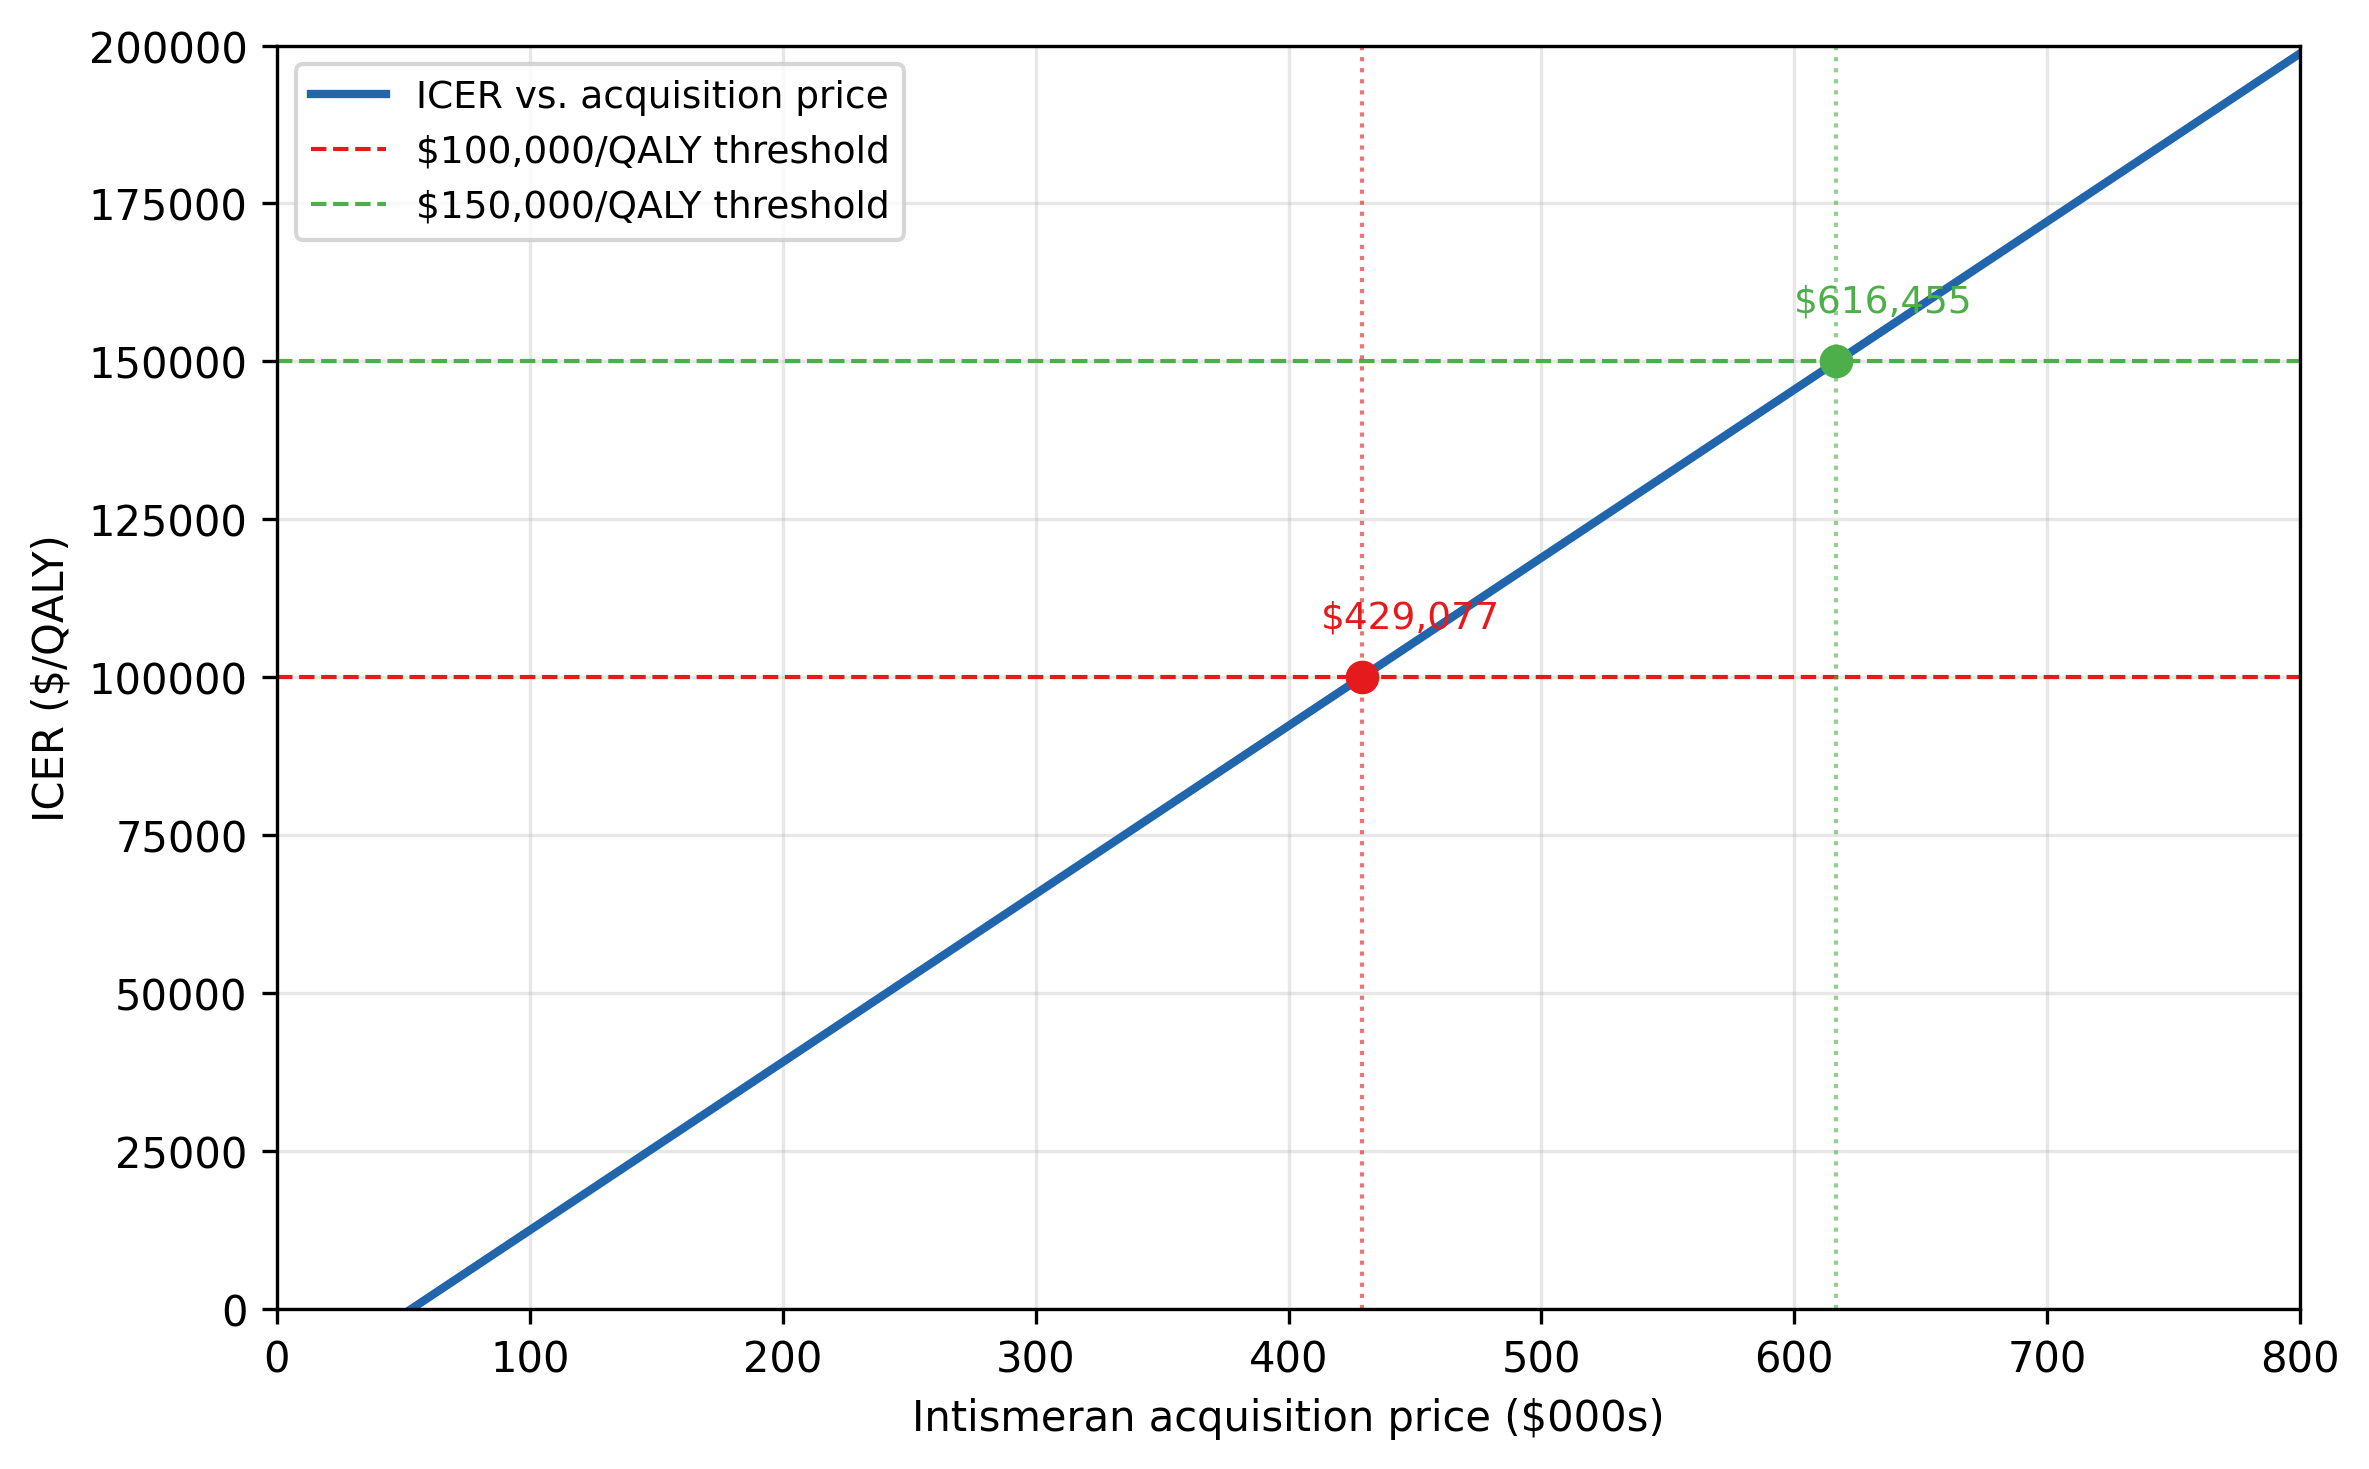
\includegraphics[width=\textwidth]{fig_s8_price_threshold.png}
\caption{ICER as a function of intismeran acquisition price. Red/green dashed lines: \$100K/\$150K thresholds. Vertical dotted lines: threshold prices.}
\label{fig:s8}
\end{figure}

% ═══════════════════════════════════════════════════
\section{Reproducibility and Reporting}
% ═══════════════════════════════════════════════════

\subsection{Technical Reproducibility}
\label{sec:tech_repro}
All analyses were performed using Python 3.12.7 (Apple Clang 15.0.0) on macOS 26.6.2 (Apple Silicon). The full code repository is available at \url{https://github.com/yichao2022/cea-intismeran} (tag \texttt{v1.0-submission}).

\textbf{Key dependencies:} NumPy 1.26.4, SciPy 1.14.1, Matplotlib 3.9.3, Pandas 2.2.3, LaTeX (TeX Live 2025, pdfLaTeX + BibTeX + natbib).

\textbf{Model details:}
\begin{itemize}
    \item Cycle length: monthly (1/12 year); time horizon: 40 years (480 cycles)
    \item Half-cycle correction: not applied (monthly cycles are sufficiently fine-grained)
    \item Discounting: continuous-time exponential: $1/(1 + r)^t$ where $r = 0.03$
    \item Random seed: 42 (PSA reproducibility)
    \item GP mortality source: US 2019 period life tables (NVSS, Arias et al. 2022)
\end{itemize}

\textbf{Code structure:}
\begin{itemize}
    \item \texttt{model.py} --- ModelParams, CEAModel (4-state PSM)
    \item \texttt{rerun\_primary.py} --- CEAModelV2 (hazard-based GP floor, waning, no-OS)
    \item \texttt{psa\_full.py} --- PSA with joint survival sampling
    \item \texttt{survival\_model\_selection.py} --- 4,096-combination model selection
    \item \texttt{final\_run.py} / \texttt{threshold\_analysis.py} --- DSA, scenarios, pricing
    \item \texttt{figures.py} / \texttt{gen\_fig\_*.py} --- Figure generation scripts
    \item \texttt{output/survival\_combos\_4096.csv} --- Full model selection results
\end{itemize}

\textbf{Data extraction:} Survival probabilities extracted from Figure~1 of Khattak et al. (2026) using WebPlotDigitizer v4.7. The digitized values are in Table~\ref{tab:s2}.

\textbf{Reproducibility:} Running \texttt{python3 rerun\_primary.py} reproduces base-case results. \texttt{python3 psa\_full.py} reproduces PSA. GitHub tag \texttt{v1.0-submission} freezes the submission code.

\subsection{CHEERS 2022 Checklist}
\label{sec:cheers}
\begin{table}[H]
\centering
\caption{CHEERS 2022 Checklist}
\label{tab:cheers}
\begin{tabular}{p{1cm}p{5cm}p{1.5cm}p{4cm}}
\toprule
\textbf{No.} & \textbf{Item} & \textbf{Reported} & \textbf{Location} \\
\midrule
1 & Title & Yes & Title page \\
2 & Abstract & Yes & Abstract \\
3 & Background & Yes & Introduction \\
4 & Health economic analysis plan & No & This is a retrospective analysis, not a pre-specified HEAP \\
5 & Model & Yes & Methods, Appendix A \\
6 & Population & Yes & Methods \\
7 & Setting & Yes & Methods \\
8 & Comparators & Yes & Methods \\
9 & Perspective & Yes & Methods \\
10 & Time horizon & Yes & Methods \\
11 & Discount rate & Yes & Methods \\
12 & Outcomes & Yes & Methods \\
13 & Health states & Yes & Appendix A \\
14 & Measurement of outcomes & Yes & Methods \\
15 & Resource use & Yes & Methods \\
16 & Currency & Yes & Methods \\
17 & Model choice & Yes & Methods \\
18 & Assumptions & Yes & Methods ({\S}2.2--2.7) \\
19 & Analytic methods & Yes & Methods ({\S}2.7) \\
20 & Study parameters & Yes & Methods ({\S}2.4, 2.5), Appendix D \\
21 & Incremental results & Yes & Results ({\S}3.1--3.2) \\
22 & Uncertainty & Yes & Results ({\S}3.4--3.6), Supplement \\
23 & Heterogeneity & Not assessed & Limitations ({\S}4.7, subgroup heterogeneity acknowledged) \\
24 & Discussion & Yes & Discussion \\
25 & Limitations & Yes & Discussion \\
26 & Funding & Yes & Declarations \\
27 & Conflicts & Yes & Declarations \\
28 & Reproducibility & Yes & Appendix \\
\bottomrule
\end{tabular}
\end{table}

\bibliography{refs}
\end{document}